% Preamble
\documentclass[12pt,twoside]{report}

\usepackage[a4paper,width=150mm,top=25mm,bottom=25mm]{geometry}

\usepackage{fancyhdr}
\pagestyle{fancy}
\fancyhead{}
\fancyhead[RO,LE]{Classification of Small Water Reservoirs with Machine Vision}
\renewcommand{\headrulewidth}{0.4pt}
\fancyfoot{}
\fancyfoot[RE,RO]{\thepage}
\fancyfoot[LE,LO]{Chapter \thechapter}
\fancyfoot[CE,CO]{Nicolas Renato Arroyo}
\setlength{\headheight}{15pt}
\renewcommand{\footrulewidth}{0.4pt}

\usepackage[utf8]{inputenc}

\usepackage{graphicx}
\graphicspath{ {figures/} }

\usepackage{float}

\usepackage{natbib}

\usepackage{caption}
\usepackage{subcaption}

\usepackage{hyperref}
\hypersetup{
    colorlinks=true,
    linkcolor=black,
    filecolor=magenta,
    urlcolor=cyan,
    citecolor=black
}
\usepackage{xurl}

\usepackage{enumitem} % For better list formatting

\usepackage{nomencl}
\makenomenclature
\usepackage{etoolbox}
\renewcommand\nomgroup[1]{%
  \item[\bfseries
  \ifstrequal{#1}{S}{Software}{%
  \ifstrequal{#1}{I}{Water Indices}{%
  \ifstrequal{#1}{M}{Machine Learning}{%
  \ifstrequal{#1}{M}{Machine Learning}{%
  \ifstrequal{#1}{D}{Data}{%
  \ifstrequal{#1}{O}{Other}{
  }}}}}}%
]}
\usepackage{amssymb}

\usepackage[table]{xcolor}

\usepackage{amsmath}

\usepackage{booktabs}

\usepackage{array}

\usepackage{microtype}

\usepackage{verbatim}

\usepackage{listings}
\definecolor{codegreen}{rgb}{0,0.6,0}
\definecolor{codegray}{rgb}{0.5,0.5,0.5}
\definecolor{codepurple}{rgb}{0.58,0,0.82}
\definecolor{backcolour}{rgb}{0.95,0.95,0.92}

\lstdefinestyle{mystyle}{
    backgroundcolor=\color{backcolour},   
    commentstyle=\color{codegreen},
    keywordstyle=\color{magenta},
    numberstyle=\tiny\color{codegray},
    stringstyle=\color{codepurple},
    basicstyle=\ttfamily\footnotesize,
    breakatwhitespace=false,         
    breaklines=true,                 
    captionpos=b,                    
    keepspaces=true,                 
    numbers=left,                    
    numbersep=5pt,                  
    showspaces=false,                
    showstringspaces=false,
    showtabs=false,                  
    tabsize=2
}
\lstset{style=mystyle}

% Start of Document
\begin{document}

\begin{titlepage}
    \begin{center}
        \vspace*{1cm}
            
        \Huge
        \textbf{Classification of Small Water Reservoirs with Machine Vision}
        
        \vspace{1.5cm}
        \Large
        Developing a Machine Vision Software Capable of Identifying and Classifying Small Farm Water Reservoirs with Satellite Imagery
                
        \vspace{1cm}
        
        
\includegraphics[width=0.4\textwidth]{contents/figures/UOM_LOGO.jpg}
        
        \vspace{1cm}
        
        \Large
        A dissertation presented to The University of Manchester for the degree of BEng (Hons) Aerospace Engineering in the Faculty of Science and Engineering

        \vfill
        \large
        Supervisor: Timothy Foster\\
        Year of Submission: 2025\\
        Student ID: 11091029\\
        Nicolas Renato Arroyo

        \vspace{1cm}
            
        \Large
        School of Mechanical, Aerospace, and Civil Engineering\\
        The University of Manchester\\
            
    \end{center}
\end{titlepage}

\title{
{Classification of Small Water Reservoirs with Machine Vision}\\
{\large The University of Manchester}\\
{
\includegraphics{UOM_LOGO.png}}
}
\author{Nicolas Renato Arroyo}
\date{\today}

\tableofcontents
\listoftables
\listoffigures
\lstlistoflistings

\newpage
\thispagestyle{plain}
\begin{center}
    \LARGE
    \textbf{Abstract}
    \vspace{0.8cm}
\end{center}
Farm water reservoirs support agriculture by storing water during high rainfall or streamflow periods for use during low periods, helping to smooth out supply-demand imbalances. Many small reservoirs in the UK are unregistered as they do not require a permit below 25\,000\,m$^3$ water capacity. It is important to have a register of these reservoirs to ensure responsible water management and to mitigate water scarcity risks. Traditional monitoring methods, such as manual surveys, are time-consuming and labour-intensive, particularly in remote areas. This project develops a machine learning software capable of classifying small water reservoirs in east England from satellite imagery.

First, the Navigable Automated Labelling Interface for Regions of Attention (NALIRA) was developed as an automated approach to generating labelled training data for machine learning models. In NALIRA, satellite images are automatically manipulated and cloud masked, then several water detection indices are calculated and plotted. The user is then prompted to label water reservoirs and water bodies in small “chunks” of the image, after which the selections are segmented and saved. NALIRA transforms the traditionally laborious task of manual image labelling into a streamlined workflow by automating data preparation, significantly accelerating training data generation. The Keras Reservoir Identification Sequential Platform (KRISP) was trained to classify small water reservoirs with the data from NALIRA.

While the development of NALIRA was more time-intensive than expected, the final software is highly modular and scalable, featuring a navigable GUI for the user to easily label large quantities of data. In total, NN small water reservoirs were found in East England, estimated with a confidence of MM\% for the period of March 2025. This area and time period were chosen for their low cloud cover and high concentration of farmland. KRISP successfully achieved XX\% accuracy, YY\% precision, and ZZ\% recall in classifying small water reservoirs, and AA\% accuracy, BB\% precision, and CC\% recall in classifying non-reservoir water bodies. 

NALIRA can be adapted to generate labelled training data for any image-based application in supervised machine learning, expediting the ground-up development of small machine vision models in engineering, medicine, and computer science. KRISP is a tool that has generated the first and only estimate of the number of small reservoirs in East England, and can therefore be used to support water management and policy decisions. 

Future work includes using more sophisticated water and cloud detection techniques, increasing quantity of training data, and a complete transition to Google Earth Engine as a data source, which would allow the program to access petabytes of web-based satellite data.


\newpage
\thispagestyle{plain}
\begin{center}
    \LARGE
    \textbf{Lay Summary}
    \vspace{0.8cm}
\end{center}

Many farms use small reservoirs to store water, which is vital for growing crops, especially during dry periods. However, countless small reservoirs across the UK aren't officially registered because they fall below a certain size limit. This lack of knowledge makes it hard to manage water resources responsibly and understand the full impact of water use in agriculture. Finding all these small reservoirs manually across the country would be incredibly time-consuming and expensive.

This project tackles this problem by using satellite images and machine learning (ML). I developed new computer software tools to automatically process satellite pictures of East England, a major farming area. One tool, named NALIRA, helps prepare the images and makes it much faster for users to identify examples of reservoirs. Another program, named KRISP, trained using these examples, then learns to automatically spot and count small reservoirs across the region.

The result is the first estimate of small reservoir numbers in East England, providing valuable information for better water management planning and environmental monitoring. The image preparation tool developed could also speed up similar ML projects in other fields that rely on analysing images.

\chapter*{Declaration}


I, Nicolas Arroyo, certify that this dissertation is my own original work unless referenced clearly to the contrary and all of the work referred to in this dissertation has been submitted in support of the degree qualification for BEng Aerospace Engineering (Hons) at The University of Manchester.

\chapter*{Intellectual Property Statement}
\begin{enumerate}[label=\roman*.]
    \item The author of this dissertation (including any appendices and/or schedules) owns certain copyright or related rights in it (the “Copyright”) and has granted The University of Manchester certain rights to use such Copyright, including for administrative purposes.

    \item Copies of this dissertation, either in full or in extracts and whether in hard or electronic copy, may be made only in accordance with the Copyright, Designs and Patents Act 1988 (as amended) and regulations issued under it or, where appropriate, in accordance with licensing agreements which the University has entered into. This page must form part of any such copies made.

    \item The ownership of certain Copyright, patents, designs, trademarks and other intellectual property (the “Intellectual Property”) and any reproductions of copyright works in the dissertation, for example graphs and tables (“Reproductions”), which may be described in this dissertation, may not be owned by the author and may be owned by third parties. Such Intellectual Property and Reproductions cannot and must not be made available for use without the prior written permission of the owner(s) of the relevant Intellectual Property and/or Reproductions.

    \item Further information on the conditions under which disclosure, publication and commercialisation of this dissertation, the Copyright and any Intellectual Property and/or Reproductions described in it may take place is available in the University IP Policy, in any relevant Dissertation restriction declarations deposited in the University Library, and The University Library’s regulations.
\end{enumerate}



% Data
\nomenclature[D]{\({TCI}\)}{True Colour Image}
\nomenclature[D]{\({RGB}\)}{Red Green Blue}
\nomenclature[D]{\({QI}\)}{Quality Indicator}

% Indices
\nomenclature[I]{\({NDWI}\)}{Normalised Difference Water Index}
\nomenclature[I]{\({MNDWI}\)}{Modified Normalised Difference Water Index}
\nomenclature[I]{\({AWEI-SH}\)}{Automated Water Extraction Index - Shadowed Regions}
\nomenclature[I]{\({AWEI-NSH}\)}{Automated Water Extraction Index - Non-Shadowed Regions}

% Machine Learning
\nomenclature[M]{\({ML}\)}{Machine Learning}
\nomenclature[M]{\({MLC}\)}{Maximum Likelihood Classifier}
\nomenclature[M]{\({SVM}\)}{Support Vector Machine}
\nomenclature[M]{\({RF}\)}{Random Forest}
\nomenclature[M]{\({KS}\)}{Keras Sequential}
\nomenclature[M]{\(FMask\)}{Function of Mask}


% Other
\nomenclature[O]{\({CPU}\)}{Central Processing Unit}
\nomenclature[O]{\({GPU}\)}{Graphics Processing Unit}
\nomenclature[O]{\({ESA}\)}{European Space Agency}
\nomenclature[O]{\({NASA}\)}{National Aeronautics and Space Administration}
\nomenclature[O]{\({NaN}\)}{Not a Number}
\nomenclature[O]{\({MB}\)}{Megabyte}
\nomenclature[O]{\({GB}\)}{Gigabyte}
\nomenclature[O]{\(GUI\)}{Graphical User Interface}
\nomenclature[O]{\({ROI}\)}{Region of Interest}
\nomenclature[O]{\(API\)}{Application Programming Interface}


% Software Names
\nomenclature[S]{\(NALIRA\)}{Navigable Automated Labelling Interface for Regions of Attention}
\nomenclature[S]{\(KRISP\)}{Keras Reservoir Identification Sequencing Platform}
\nomenclature[S]{\(IPDMP\)}{Individual Project Data to Model Pipeline}
\nomenclature[S]{\(KRISP-Y\)}{Keras Reservoir Identification Sequencing Platform - Yield}

\printnomenclature

\chapter{Introduction}


\section{Overview}
The agriculture industry is highly reliant on water for crop production and food supply. Around 70\% of fresh water used globally is used for agriculture \citep{emily_2023}, and farms depend on reliable water supply to irrigate crops regularly and ensure that their supply meets the industry's demand. Severe rainfall variability damages not only a farmer's yield and agricultural output, but also a household's dietary diversity \citep{object_object_2020}, which is necessary for proper "nutrition and overall well-being" \citep{food_diversity}.

Rainfall variability has been shown to "frequently undermine farm yields, reduce food availability, and lower income" \citep{guido_zimmer_lopus_hannah_gower_waldman_krell_sheffield_caylor_evans_2020}. This is not limited to periods of low rainfall, but also periods of high rainfall, which can "increase agricultural runoff", "harm water quality", and hamper crop production by damaging the soil on which they are grown. These problems are only exacerbated as climate change becomes an increasingly pressing issue \citep{united_states_environmental_protection_agency_2025} and rainfall variability is increased. For farmers in area of high water volatility, the need for reliable information on water levels is growing. 

By enabling farmers to capture and store water during periods of high availability (such as winter rainfall or peak streamflow), these reservoirs provide a vital supply for irrigation and other needs during drier periods, effectively smoothing seasonal supply-demand imbalances caused by rainfall variability. This reduces reliance on potentially costly mains water or direct abstraction during sensitive summer months, offering greater protection against drought and supporting consistent crop production.

In the UK, small farm water reservoirs under 25,000 cubic metres \citep{ukgov_2014_reservoirs} do not require permits. This could raise potential risks to the environment, as with more non-permit, non-registered water reservoirs, there are more likely to be adverse effects on the local water cycle due to unpredictable levels of water abstraction being carried out. For this reason, it would be beneficial for governments to have the ability to map these small farm water reservoirs. One method of doing this is through analysis of satellite data with a classification model able to identify and note the size and location of water reservoirs, particularly in east England. 

Recognising the importance of this on-farm infrastructure for both food security and environmental management, UK government policy initiatives actively encourage the development of water storage solutions. Schemes like the Water Management Grant, part of the Farming Investment Fund, offer financial support to farmers for constructing reservoirs and investing in efficient irrigation systems \citep{ruralpaymentsagency_2023}, aiming to promote sustainable water use. These initiatives align with broader governmental goals, such as Defra's aim to significantly increase the amount of water stored by the farming sector by 2050 \citep{andcornwall_2024}. Additionally, collaborative approaches like multi-farm reservoirs and water sharing schemes \citep{for_2024} are being explored through dedicated funding to further enhance regional water management resilience.

\section{Problem Addressed}
While many large water reservoirs and water abstraction operations are licensed and monitored, a significant data gap exists regarding the prevalence and distribution of small, unregistered reservoirs on UK farms. This lack of knowledge is problematic for several key reasons. Firstly, without a comprehensive register of these smaller reservoirs, it becomes impossible to accurately assess the true uptake of on-farm water storage solutions or evaluate the effectiveness of policy initiatives designed to encourage their sustainable growth. Secondly, although individual small reservoirs fall below regulatory thresholds and may primarily fill during wetter periods, their cumulative impact is unknown. Unmonitored proliferation could potentially lead to significant alterations in local hydrological cycles and unforeseen environmental sustainability issues, even if individual abstractions seem minor. Finally, this data gap hinders effective water resource management and regulatory oversight. If the locations and number of these reservoirs are unknown, authorities cannot verify whether abstraction rules, such as permitted filling times, are being adhered to, potentially undermining efforts to manage water resources sustainably, especially given that some abstraction practices are already known to be unsustainable \citep{departmentofenvironmentfoodandruralaffairs_2019_abstraction}.

To ensure responsible retention, usage, or disposal of immediate-use abstracted and reservoir-stored water, it is first necessary to have an accurate register of the reservoirs in the country. Travelling to each farm and identifying whether or not they use a water reservoir is a costly and time-consuming endeavour. Additionally, these types of visits would have to be regular enough so that the filling and release of water can be monitored as well. For a resource and staff-constrained agency such as the Environmental Agency (EA), \citep{comptrollerandauditorgeneral_2022}, it is impossible to have enough enforcers to go out checking every farm. This problem is further exacerbated by the steadily declining funding the the EA has been receiving in recent years demonstrated in figure \ref{fig:EA funding decline}. 

\begin{figure}[ht]
    \centering
    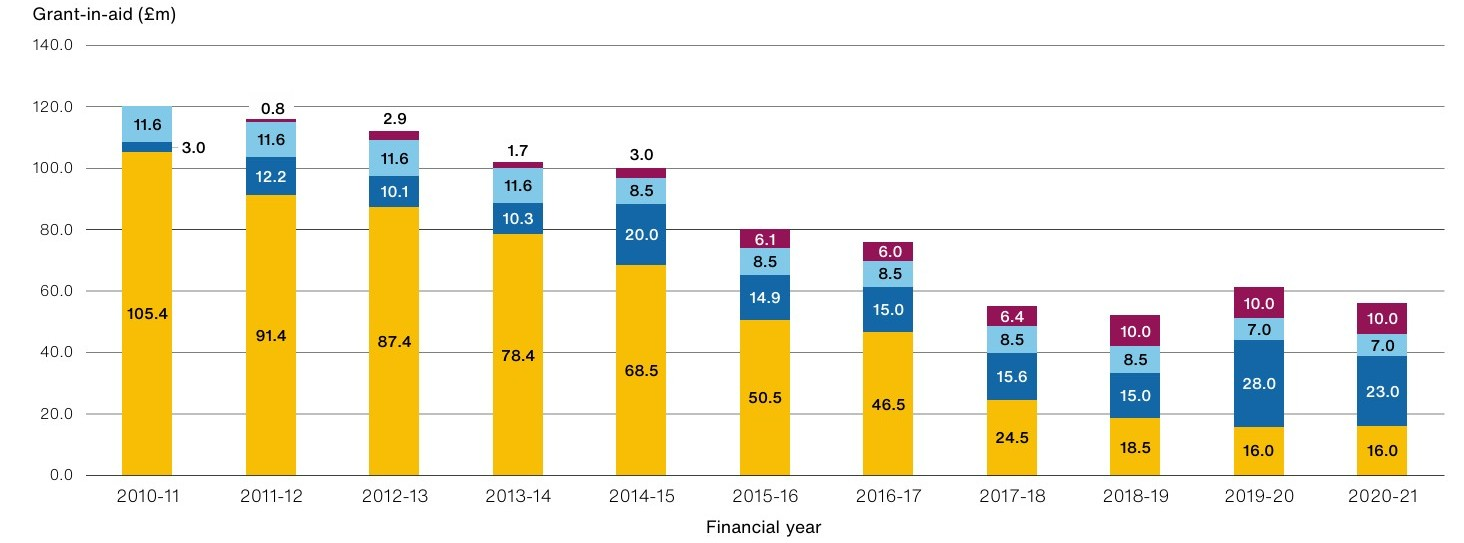
\includegraphics[width=0.5\linewidth]{contents/figures/intro-environment agency funding.jpg}
    \caption{"Grant-in-aid funding to the Environment Agency for environmental protection, 2010-11 to 2020-21" \citep{comptrollerandauditorgeneral_2022}}
    \label{fig:EA funding decline}
\end{figure}

Given the challenges and potential inaccuracies associated with ground-based monitoring for numerous small, unregistered reservoirs, alternative approaches are needed. Satellite remote sensing, the science of acquiring information about the Earth's surface by "measuring reflected and emitted radiation at a distance" \citep{usgs_2022a}, offers significant potential as a monitoring tool, providing wide-area coverage repeatably and often more cost-effectively than extensive field surveys, especially for monitoring change over time. However, raw satellite imagery requires sophisticated analysis to extract meaningful information.

Therefore, it would be beneficial to develop specialised algorithms capable of processing these datasets to automatically identify potential water reservoirs on farms. Critically, such algorithms must go beyond simple water detection; the model should also be able to differentiate water body features that resemble, and are most likely to be, constructed farm reservoirs from other water bodies (like rivers, ponds, or flooded areas) and non-water features that might appear spectrally similar. Furthermore, for these advanced remote sensing methods to be truly impactful, the development of robust algorithms must be accompanied by accessible tools and clear methodologies. This is essential to translate complex satellite data and model outputs into practical, actionable information that can be readily used by policymakers, regulatory bodies like the Environment Agency, and water resource managers to monitor reservoir distribution, assess compliance, and evaluate the effectiveness of water management policies.

The main beneficiary for this project is likely to be a government body seeking to identify unpermitted reservoirs that pose potential risks to the water cycle or nearby ecosystems. 

\section{Aim and Objectives}
The aim for this project is to investigate the quantity, location, and size of small farm water reservoirs in the east of England. To do this, I will develop and train a machine learning classification model that uses satellite imagery data to identify water reservoirs. The model should also be able to differentiate water reservoirs from other non-reservoir water bodies. The remaining third class will be composed of land types that contain neither. 

I have defined four objectives that shall be achieved to ensure successful development and training of the classification model: 
\begin{enumerate}
    \item Select one appropriate satellite image for the development of the necessary software tools and three more satellite images for model deployment. 

    The singular development image is intended for building the programs around a generic satellite image (specifically Sentinel 2), while the three deployment images are for validating the program under different conditions. 
    \item Develop a software tool to automate satellite imagery handling/pre-processing and facilitate the semi-automated creation of labelled training data through a dedicated user interface. 
    
    Satellite imagery handling includes automatic file search given a directory, cloud masking, index calculation, data file preparation, and response data saving. 
    \item Build, train, and validate a machine learning classification model (specifically using the Keras Sequential model) for water reservoirs, non-reservoir water bodies, and land.
    \item Deploy the model over East England and produce a map of the quantity, location, and size of all water reservoirs in East England for March 2025. 
\end{enumerate}

The following section will explain and justify the study area and time period selected for these objectives.

\section{Study Area and Time Period}
As can be seen from the final objective, the study area is East England, and the time period was selected as the month of March in 2025. 

This study area was selected because East England, together with the East Midlands, contributes the highest total income from farming in the UK \citep{defra_2024}, indicating the greatest density of agricultural holdings and thus the most small reservoirs to detect. Moreover, East Anglia is among the driest regions of the country \citep{matthew_de-machen_mjr.global_2024} and already under acute pressure from summer water shortages; it accounts for the highest irrigation abstractions in England and Lincolnshire, and its farms are most exposed to drought risk \citep{ukia_2024, johns_2023}. 

Climate projections and recent observations signal widening supply–demand gaps: by 2050, summer water deficits in England could approach five billion litres per day during dry spells, potentially triggering hosepipe bans and prioritisation conflicts between public supply and agriculture \citep{horton_2024}. Concurrently, modelling under a range of socio-economic and climate scenarios, forecasts estimate that irrigation demand in East Anglia may rise 10 to 40 percent by 2050, driven by hotter, drier summers and evolving cropping patterns \citep{henriques_holman_audsley_pearn_2008, uk_ceh_2025}. 

These intersecting factors, high farm density, the driest UK climate, and escalating water use demands, make East England the ideal test-bed for an automated reservoir-mapping tool that supports regional water‐management and drought‐resilience planning.

This time period was finalised and selected to simplify data handling was much as possible. March 2025 was "the sunniest March" since records began \citep{pressoffice_2025_a}, making it ideal for satellite imagery. Clouds in satellite imagery are problematic because they can largely obscure important information on the ground. There are some strategies to mitigate these problems, which will be covered in the Methodology section, however the simplest way to avoid the problem altogether is to select images with the lowest cloud cover percentage. Selecting March as the month of choice is optimal as it guarantees a larger proportion of the images selected will be only minimally covered by clouds. 

\subsection{To what extent is this problem global?}
While this study focuses on East England as a case study/proof-of-concept, the problem of needing to efficiently identify and monitor small water reservoirs is a widespread global challenge relevant to agriculture, environment, and water management. This study demonstrates a scalable technical solution using globally available data and techniques, proving that this machine learning approach can be effectively implemented to tackle this global problem.

\section{Dissertation Structure}
I will now provide a brief overview of the contents of each section in this report. 
\subsection{Literature Review}
\subsection{Methodology}
\subsection{Results}
\subsection{Discussion}
\subsection{Conclusion}

\chapter{Literature Review}


This literature review serves to provide the essential technical and theoretical background underpinning the methodology employed in this thesis. It delves into the core concepts and established techniques within the fields of remote sensing and machine learning that are pertinent to this research for the identification and classification of small water reservoirs from satellite imagery. By reviewing the relevant literature in this field, I will pinpoint the precise knowledge gap, namely the absence of a validated, end-to-end pipeline tailored for high-resolution detection of small farm reservoirs in East England.

The following sections build on this foundation:
\begin{enumerate}
    \item \textbf{Remote Sensing for Water Body Mapping} - Why optical satellites (Sentinel-2, Landsat) are ideal for small-reservoir mapping, comparing their spatial, spectral and revisit capabilities.
    \item \textbf{Water Detection Methods} - Techniques for isolating water pixels including classic, numerically computed indices (NDWI, MNDWI, AWEI-NSH/SH), traditional classifiers (SVM, Maximum Likelihood), and deep-learning algorithms.
    \item \textbf{Cloud Detection and Masking} - From simple quality-flag masks to Fmask’s object-based approach and OmniCloudMask’s sensor-agnostic neural model, and how each handles cloud/shadow errors.
    \item \textbf{Machine Learning Algorithms} - Overview of unsupervised clustering versus supervised learning, with a comparison focused on the practical applications of Random Forest and Keras Sequential.
    \item \textbf{Machine Learning and Water Classification}
    \begin{enumerate}
        \item How supervised methods have been applied to remote-sensing water detection.  
        \item Key case studies of reservoir mapping, and where existing pipelines still fall short.
    \end{enumerate}
\end{enumerate}

By reviewing these interconnected topics, this literature review aims to build a comprehensive understanding of the technical landscape, providing the necessary foundation for the methodology developed and applied in this thesis.

\section{Remote Sensing for Water Body Mapping}
\subsection{What is Remote Sensing?}
Remote sensing is the practice of acquiring information about the Earth's surface without direct contact, typically through sensors mounted on satellites or aircraft \citep{usgs_2022a}. By capturing the reflected or emitted electromagnetic radiation from land, water, and atmosphere, remote sensing provides systematic, repeatable, and scalable observations across large areas.

For the task of small reservoir detection, optical satellite imagery is particularly well-suited. Optical sensors measure reflected solar radiation in visible, near-infrared, and shortwave-infrared wavelengths, enabling strong discrimination between surface water and surrounding land cover based on spectral signatures. Water bodies typically appear darker in the near-infrared and shortwave-infrared bands compared to vegetation, soil, or built-up areas, making them distinguishable through simple band ratios or more advanced machine learning methods.

\subsection{Satellite Options}
There are several options for optical satellites currently in operation. The first requirement for this study is that the data must be freely available, otherwise it would be unfeasible to scale the project globally without significant monetary investment. This means that the ultra-high resolution satellite imaging platforms such as MAXAR are not option as they are privately run and therefore have costs for their use. The two main remaining options are to use Sentinel, the European Space Agency (ESA) satellites, or Landsat, the NASA satellites, both of which are publicly funded and host freely accessible data.

The Sentinel 2 constellation is made up of three satellite: Sentinel 2A, 2B, and 2C, with the Sentinel 2A, the first to be launched, operating since 2015 \citep{esa_2024}. Each satellite has functionally the same sensors and specifications, so whenever "Sentinel 2" is mentioned in this thesis, this is used as an umbrella term to mean any of the three Sentinel 2 satellites. These satellites have a maximum spatial resolution of 10m, with file options for 20m and 60m files. 

Landsat 7 has been operating since 1999, however due to the failure of a component called the Scan Line Corrector in 2003, images have had "gaps" in them \citep{usgs_2024}. Landsat 8 and 9 operate as intended and have been in orbit since 2013 and 2021 respectively \citep{usgs_2023, usgs_2022}. These satellites have a maximum spatial resolution of 30m, which is considerably less fine than the Sentinel 2 options. For this reason, many researchers prefer to use Sentinel images over Landsat as the additional detail afforded by Sentinel is necessary for many applications \citep{ghansah_2022_monitoring, kirby_ferguson_rennie_cousineau_nistor_2024}. 

\subsection{Resolution}
There are two different kinds of resolution to consider when discussing remote sensing data. The first is the regular, pixel resolution, just like the one on televisions, and computer or phone screens. This resolution is calculated from the product of the number of pixels on each length of the image, so an image with 1920 pixels along its length and 1080 pixels along its width has a 1920x1080 resolution, and a total pixel count of 2,073,600. This is also known as "full HD" \citep{lenovo_2021}. 

The second kind of resolution is specific to satellite imagery and it is known as "spatial resolution". This is defined as the "scale or size of the smallest unit of an image capable of distinguishing objects" \citep{zhang_li_zhang_li_2023}. When we say "10 metre resolution", this means the spatial resolution of satellite image, meaning each pixel on the image represents a 10m by 10m area on the ground. 

Technically speaking, resolution is defined by the peaks of the reflecting light from an object not overlapping with the nearest light-reflecting object that can be resolved as well. This is shown in figure \ref{fig:LR resolution graph} and this principle applies to various fields of optical imaging. 

\begin{figure}[ht]
    \centering
    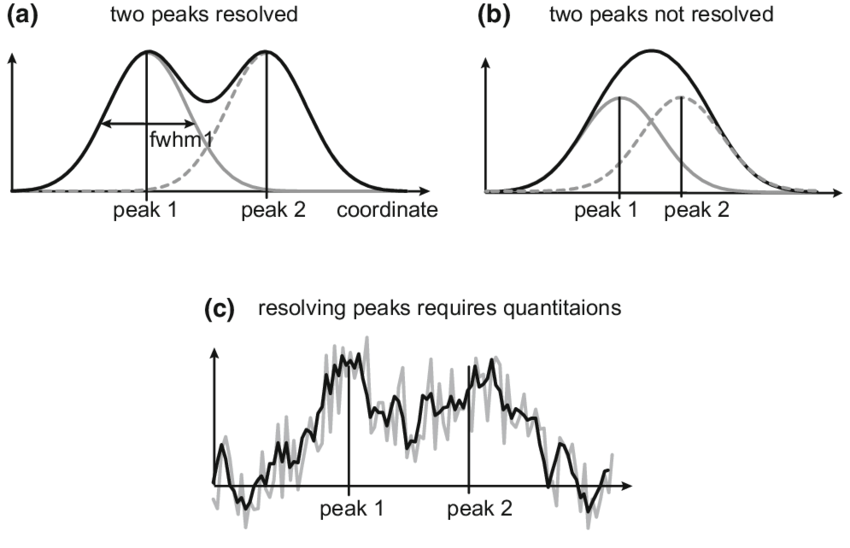
\includegraphics[width=0.6\textwidth]{contents/figures/LR resolution peaks.jpg}
    \caption{Graphical representation of resolution \citep{kudryashev_2018}}
    \label{fig:LR resolution graph}
\end{figure}

It is important to note that satellite images have a spatial resolution but they also have a regular pixel resolution. For example, the highest resolution Sentinel 2 satellite images used in the development of software for this study (the ones with 10m spatial resolution) have a pixel resolution of 10980x10980, meaning a total pixel count of 120,560,400. This very large pixel count is necessary to be able to zoom in very close to see small features on the ground for Sentinel 2 satellites, which orbit at 786 km \citep{esa_2023}. 

\subsection{Optical Sensors}
There are thirteen optical imaging sensors on the Sentinel 2 satellites \citep{sinergise_2025}. These sensors have varying spatial resolutions, ranging from 10m for the sharpest and largest images, and 60m for the smallest images with the least detail. The 60m resolution images are not detailed enough to be usable for data labelling or model training, however they are useful for fast troubleshooting as the smaller files take less time to open and manipulate. Images generated with 10m or 20m resolution are usable, however 10m resolution is preferred for easier viewing. 

\section{Water Detection Methods}
\subsection{Spectral Water Indices}
Spectral water indices play a pivotal role in distinguishing water pixels from surrounding land cover. These band-ratio techniques have become standard in operational water mapping workflows, offering enhanced contrast between water and non-water surfaces across diverse environments. 

\subsubsection{Normalised Difference Water Index}
The Normalised Difference Water Index (NDWI), introduced by \cite{mcfeeters_k_1996}, uses the green and near-infrared bands (NIR) to delineate water features from other land areas. 

\begin{equation} \label{eq-ndwi}
NDWI = \frac{\rho_{green} - \rho_{NIR}}{\rho_{green} + \rho_{NIR}}
\end{equation}

For a computer, equation \ref{eq-ndwi} means that, to calculate one pixel for a map of NDWI from a satellite image, it must take the corresponding pixel in the image for green reflectance, and the corresponding pixel in the image for NIR reflectance, and apply the equation to it. In reality, although this is the process what would be most intuitive to humans, computers perform significantly better when they take advantage of matrix-wise operations to vastly improve efficiency, so rather than calculating a NDWI array by going pixel by pixel and applying the equation to each one, computers conduct all the calculations at the same time. This same method applies for each other index that will be discussed. More details on this method will be discussed further in the methodology section. 

\subsubsection{Modified Normalised Difference Water Index}
The Modified NDWI (MNDWI) replaces the NIR band in NDWI with a short-wave infrared band (SWIR) to suppress built-up and vegetated noise \citep{xu_hanqiu_2006}. 

\begin{equation} \label{eq-mndwi}
MNDWI = \frac{\rho_{green} - \rho_{SWIR1}}{\rho_{green} + \rho_{SWIR1}}
\end{equation}

Sentinel 2 has two SWIR bands, and MNDWI specifically requires the SWIR1 band, which has a 20m spatial resolution. 

\subsubsection{Automated Water Extraction Index}
There are also some newer spectral water indices that have been used for water detection, including the Automated Water Extraction Index (AWEI) \citep{feyisa_gudina_meilby_fensholt_proud_2014b}, which has two forms: one optimised for higher-accuracy detection of water in shadowed regions, and another for unshadowed regions, AWEI-SH and AWEI-NSH respectively.

\begin{equation}
AWEI_{NSH} = 4 \times (\rho_{green} - \rho_{SWIR1}) - (0.25 \times \rho_{NIR} + 2.75 \times \rho_{SWIR2})
\end{equation}

\begin{equation}
AWEI_{SH} = \rho_{green} + 2.5 \times \rho_{blue} - 1.5 \times (\rho_{NIR} + \rho_{SWIR1}) - 0.25 \times \rho_{SWIR2}
\end{equation}

These indices are slightly more complex than NDWI and MNDWI and make use of different bands, such as the blue band, which has a 10m spatial resolution, and the SWIR2 band, which has a 20m spatial resolution. 

Both the study conceiving this index \citep{feyisa_gudina_meilby_fensholt_proud_2014b} and independent studies comparing various index performances \citep{kirby_ferguson_rennie_cousineau_nistor_2024} have shown that AWEI, specifically AWEI-NSH generally outperforms the other methods of spectral index water delineation. 

\subsection{Traditional Machine Learning Methods}
Another method of identifying water pixels in an image is to use machine learning (ML). The algorithms discussed in this sub-section are both supervised algorithms, meaning they ingest labelled training data and output a prediction on the class of each pixel in an image. These types of algorithms are significantly more complex than a simple spectral water index as they require training and often precise fine-tuning for optimal results \citep{vapnik_vladimir_n_1997}. However, ML algorithms are also often more accurate when trained on enough data. ML algorithms can model complex, multi-feature relationships for higher accuracy, while indices use simpler, although often significantly faster formulas based on fewer spectral bands.

\subsubsection{Support Vector Machine}
Support Vector Machine (SVM) is a supervised ML algorithm with the goal being to find an optimal hyperplane that best separates data points belonging to different classes in a high-dimensional space \citep{berwick_2003}. A hyperplane is essentially a decision boundary; in 2D, it is a line, in 3D it is a plane, and in higher dimensions, it is a hyperplane \citep{ktena_sotiras_ferrante_schirmer_arichi_chung_2023}. It maximises the margin between the hyperplane and the nearest points (support vectors) for robust classification.

SVM has been tested on accuracy of water detection, \citep{maity_2016} as well as vegetation and urban areas. 

\begin{table}[ht]
    \centering
    \begin{tabular}{|l|c|c|c|}
        \hline
        CLASS & Urban & Vegetation & Water \\
        \hline
        Urban & 72.53 & 0.25 & 27.22 \\
        Vegetation & 0 & 97.70 & 2.30 \\
        Water & 10.53 & 6.17 & 83.30 \\
        \hline
    \end{tabular}
    \caption{SVM Confusion Matrix \citep{maity_2016}}
    \label{tab:LR SVM confusion matrix}
\end{table}

In table \ref{tab:LR SVM confusion matrix}, the numbers along the diagonal (i.e. the where "urban" meets "urban", the cell where "vegetation" meets "vegetation", and the cell "water" meets "water") show the correct predictions made by the SVM model, or true positives, whereas the ones off the diagonal show misclassification, or false positives. While SVM has a high accuracy, as is shown by the values along the diagonal, the best application for it seems to be in identifying vegetation, where it achieves up to 97.7\% accuracy with relatively few false positives and false negatives. However, when identifying water, the accuracy falls to 83.3\%, with false negatives and false positives reaching up to 27.2\%. 

\begin{itemize}
    \item \textbf{Advantages:}
    \begin{itemize}
        \item Effectively handles high-dimensional data and complex non-linear separations using kernels.
        \item Often achieves greater accuracy, particularly where features have similar spectral responses.
    \end{itemize}
    \item \textbf{Disadvantages:}
    \begin{itemize}
        \item Requires labelled training data and significant computational resources, especially for training.
        \item Can be less interpretable and needs careful parameter tuning compared to simple index thresholds.
        \item More complex implementation, especially over spectral indices.
    \end{itemize}
\end{itemize}

\subsubsection{Maximum Likelihood Classifier}
Similarly to SVM, the Maximum Likelihood Classifier (MLC) is a supervised ML algorithm. MLC uses probability distributions to assign data points a class. It assumes data within each class follows a normal distribution and uses training data to estimate the probability parameters for each class \citep{arcmap_2021}. 

In remote sensing specifically, MLC classifies pixels in satellite imagery by calculating the probability that the pixel's spectral signature belongs to each predefined land cover class, assigning it to the most probable one.

\begin{itemize}
    \item \textbf{Advantages:}
    \begin{itemize}
        \item Considers class variability (variance-covariance) across all input bands, often yielding robust results.
        \item Provides quantitative probability values for pixel assignment to each class.
    \end{itemize}
    \item \textbf{Disadvantages:}
    \begin{itemize}
        \item Requires training data and more computational resources.
        \item Assumes normal distribution for class data, which can limit accuracy if untrue.
        \item Sensitive to the quality and representativeness of training data; poorly defined training sites significantly impact results.
        \item Also more complex to implement than spectral indices.
    \end{itemize}
\end{itemize}

\subsection{Deep Learning Methods}
\subsubsection{OmniWaterMask}
OmniWaterMask is a Python library designed for high-accuracy water segmentation in satellite imagery \citep{dpird-dma_2024}. It supports imagery from various satellites, crucially Sentinel 2, but also higher resolution options such as MAXAR, and is built on data from the Red, Green, Blue, and NIR bands. Importantly, these are the four bands on Sentinel 2 that have access to the 10m resolution sensors. 

The documentation for OmniWaterMask claims it provides "high accuracy" water segmentation. However, unlike other products for deep learning solutions to remote sensing problems from the Department of Primary Industries and Regional Development \citep{wright_2025}, OmniWaterMask does not yet have scientific paper published to evaluate its accuracy. As a result, this approach has not been compared to any other approaches such as spectral index water detection or traditional machine learning, meaning that a direct quantitative comparison of OmniWaterMask's accuracy is not available.

\subsection{Resolution Considerations}
It is important to note that the selection of the "best" index for this project does not solely depend on the accuracy with which the index can delineate boundaries of water or total area. A large part of this project is made up of data labelling and training point digitisation, meaning that the viewing experience should be taken into account. 

Only four of the thirteen optical imaging sensors on Sentinel 2 can achieve the maximum 10m spatial resolution: Band 2 (blue), Band 3 (green), Band 4 (red), and Band 8 (near-infrared). 

\begin{table}[ht]
\centering
\begin{tabular}{|c|c|c|c|}
\hline
\textbf{Band} & \textbf{Label} & \textbf{Wavelength (nm)} & \textbf{Resolution (m)} \\
\hline
1 & Aerosol & 443 & 60 \\
\rowcolor{yellow} 2 & Blue & 490 & 10 \\
\rowcolor{yellow} 3 & Green & 560 & 10 \\
\rowcolor{yellow} 4 & Red & 665 & 10 \\
5 & Red Edge & 705 & 20 \\
6 & Red Edge & 740 & 20 \\
7 & Red Edge & 783 & 20 \\
\rowcolor{yellow} 8 & NIR & 842 & 10 \\
8A & Narrow NIR & 865 & 20 \\
9 & Water Vapour & 945 & 60 \\
10 & SWIR Cirrus & 1375 & 60 \\
11 & SWIR 1 & 1610 & 20 \\
12 & SWIR 2 & 2190 & 20 \\
\hline
\end{tabular}
\caption{Sentinel 2 Spectral Bands Information \citep{sinergise_2025}}
\label{tab:LR s2 band wavelengths and resolutions}
\end{table}

As will be covered in more depth in the methodology section, the way that spectral indices must be calculated involves ensuring all arrays converted from an image must be of the same size. This means that, if an index is calculated using two bands of different resolutions, the lower resolution band takes precedent, resulting in a lower resolution image. Given that MNDWI, AWEI-SH, and AWEI-NSH all require at least one band with 20m resolution, every image generated displaying any of these water will have roughly half the resolution of an image generated using NDWI. This is because NDWI uses only the green and NIR bands, both of which are supported with 10m resolution. 

\begin{figure}[ht]
     \centering
     \begin{subfigure}[b]{0.45\textwidth}
         \centering
         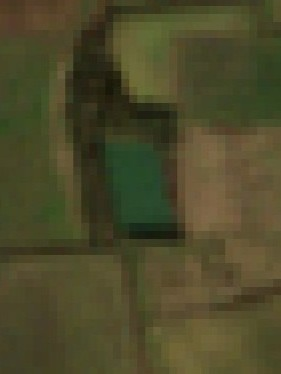
\includegraphics[width=\textwidth]{contents/figures/LR 10m res.jpg}
         \caption{10m Resolution Example}
         \label{fig:10m resolution example}
     \end{subfigure}
     \hfill
     \begin{subfigure}[b]{0.45\textwidth}
         \centering
         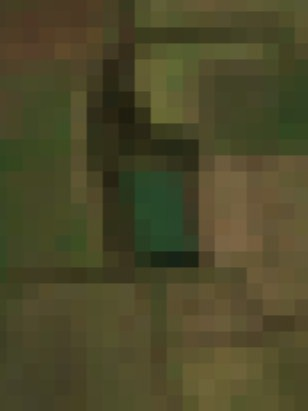
\includegraphics[width=\textwidth]{contents/figures/LR 20m res.jpg}
         \caption{20m Resolution Example}
         \label{fig:20m resolution example}
     \end{subfigure}
        \caption{10m (left) vs 20m (right) Resolution Comparison for a True Colour Image (TCI)}
        \label{fig:lit review resolution comparison}
\end{figure}

A higher resolution image is sharper and clearer than one with lower resolution, as can be seen from figure \ref{fig:lit review resolution comparison} comparing the appearance of a reservoir in a 10m spatial resolution image against a 20m spatial resolution image. This makes it easier to spot small details on a screen, as well as having the advantage of reducing eye strain when looking at screens for a long time \citep{klein_2024}. Given that the data labelling and training point digitisation process involves careful observation of these images on computer screens for extended periods of time, an index capable of accessing higher resolutions is a non-trivial consideration. Additionally, as this project is concerned with the detection of small reservoirs, it is most natural to give priority to the images that have the most information in them. 

Therefore, although not explicitly related to the performance of the index, NDWI does have the resolution advantage over the other indices.

\subsection{Summary}
Studies by \cite{kirby_ferguson_rennie_cousineau_nistor_2024} comparing water detection performance across spectral indices and machine learning methods found that, while no single index is universally best for identifying water in satellite imagery, AWEI-NSH performed most successfully in the tested study locations. MNDWI did not perform as well as NDWI in many cases, and the AWEI-SH index performed worse than AWEI-NSH in general as well. 

Out of the machine learning methods, SVM was the most performant overall, however MLC was better suited for delineating areas of water, rather than boundaries. This is important for the application in this project because it is concerned with spotting water reservoirs, which would benefit from identifying an area, rather than identifying the delineation from water to land, for example. 

To help visualise the basic sensitivity analysis conducted for selecting which method to select, table \ref{tab:water detection comparisons} shows each method of water detection discussed along with the expected complexity of implementation and the expected effectiveness of the method at detecting water once implemented, based on the quantitative comparative study by \cite{kirby_ferguson_rennie_cousineau_nistor_2024}.

\begin{table}[ht]
\centering
\begin{tabular}{|c|c|c|c|}
\hline
\textbf{Method} & \textbf{Type} & \textbf{Complexity} & \textbf{Effectiveness} \\
\hline
Spectral Index & NDWI & Simple & Moderate \\
Spectral Index & MNDWI & Simple & Low \\
Spectral Index & AWEI-SH & Simple & Moderate \\
Spectral Index & AWEI-NSH & Simple & High \\
Traditional ML & SVM & High & High \\
Traditional ML & MLC & High & Moderate \\
Deep Learning & OmniWaterMask & High & Unverified \\
\hline
\end{tabular}
\caption{Comparison of different water detection methods in expected complexity of implementation and expected effectiveness}
\label{tab:water detection comparisons}
\end{table}

Given that each of the spectral indices are simple equations and Python's integration with NumPy makes large matrix-wise operations very efficient and straightforward, it is logical that their implementation would be straightforward as well. This will be discussed further in the methodology section. 

Although MLC uses more advanced probability measures to produce a likelihood that a given pixel is or is not water, spectral indices produce high or low values depending on how much of the required wavelengths are reflected. This could behave as a kind of "confidence" or likelihood that a given pixel is water. 

The deep learning and traditional machine learning methods, however, are much more complex, and would require significant time investment to fully understand and apply properly. 

\section{Cloud Detection and Masking}
Clouds and their shadows can be misclassified as water bodies or reservoirs, so cloud contamination presents one of the potential obstacles in optical water mapping. There are several possible approaches of varying complexity and effectiveness when considering optimal methods of cloud masking. 

\subsection{QI Correspondence Method}
The most basic method makes use of the "Quality Indicator" (QI) files stored in each Sentinel 2 image \citep{gatti_bertolini_carriero_2015}. These files are "XML reports including Quality Indicators, GML Quality Mask files and JP2 Preview Image file". One of the quality mask files named "MSK\_CLDPRB\_20m" contains data for each pixel on the likelihood of that pixel being a cloud pixel. This likelihood is expressed as a float number between 0 and 1, 0 being not a cloud, and 1 being almost assuredly a cloud. 

By using these files to eliminate the corresponding pixels in the band images, we can  conduct basic cloud masking. This approach is basic, but very easy to implement, making it likely well-suited for a study where cloud cover is low. 

As there was no previous literature on this masking method, I have named it the "QI Correspondence" method as it stores cloud pixel positions using the QI cloud masking file, and then eliminates the corresponding pixel in the band images by converting it to a \texttt{Not a Number} (\texttt{NaN}).

\subsection{FMask}
Although initially designed exclusively for Landsat, \cite{frantz_haß_uhl_stoffels_hill_2018} was able to replace the missing thermal imaging sensor required for Landsat, enabling FMask to be adapted for Sentinel. The Fmask algorithm and its subsequent versions have set the benchmark for automated, object-based cloud and cloud-shadow detection in Landsat imagery \citep{qiu_zhu_he_2019}. 

The Fmask (Function of mask) algorithm is a single-date, object-based method for detecting clouds and their shadows in optical satellite images \citep{tarrio_tang_masek_claverie_ju_qiu_zhu_woodcock_2020}. It first uses a series of spectral tests, examining the reflectance characteristics that distinguish clouds from land and water, and computes a cloud probability layer based on measures of brightness and how much the spectrum varies. Pixels flagged as potential clouds are then grouped into spatial objects, and the algorithm uses thermal measurements to estimate each cloud’s height \citep{zhu_helmer_2018}. By projecting the three-dimensional shape of each cloud along the sun’s path, Fmask defines where its shadow should fall, and then confirms actual shadow pixels by looking for darker targets in those areas. In the same pass it also identifies snow and water bodies using additional spectral criteria. The result is a per-pixel map assigning each location to one of five classes: clear sky, cloud, cloud shadow, snow, or water. Downstream workflows then use these classes to restrict analysis to clear-sky pixels and thus greatly reduce errors when extracting water bodies. 

\subsection{OmniCloudMask}
OmniCloudMask is built around a deep convolutional neural network that learns to label each pixel as either clear sky, clouded, or under the shadow of a cloud \citep{wright_duncan_nik_thompson_george_2024}. During training, the input patches of red, green and near-infrared bands are first spectrally normalised and then randomly resampled to resolutions between ten and fifty meters. This “mixed-resolution” approach allows the network to be trained on the spectral and spatial characteristics of both medium and high resolution sensors. 

The model’s final layers perform a three-way classification on each pixel, and new images are normalised and resized then fed into the network in overlapping tiles. This allows the model to be trained on features that do not depend on the sensor's characteristics, meaning that it can make predictions on data from a very wide range of satellite imaging platforms without needing to be trained individually to that platform. 

\subsection{Summary}
The FMask and OmniCloudMask algorithms are built on sophisticated and long-standing platforms which are being constantly maintained. This allows them to offer higher accuracy than the basic QI Correspondence method, however this comes at the cost of more complex implementation and computationally expensive operations. 

\begin{table}[ht]
\centering
\begin{tabular}{|c|c|c|c|}
\hline
\textbf{Method} & \textbf{Type} & \textbf{Complexity} & \textbf{Effectiveness} \\
\hline
QI Correspondence & Numerical & Simple & Unverified \\
FMask & MNDWI & Moderate & High \\
Deep Learning & OmniCloudMask & Moderate & Moderate \\
\hline
\end{tabular}
\caption{Comparison of different cloud masking methods in complexity of implementation and expected effectiveness}
\label{tab:cloud masking comparisons}
\end{table}

The QI Correspondence method is very simple and easy to implement but likely does not offer particularly high accuracy. However, for the specified month of March 2025, having very low cloud cover, a high-accuracy model may not be required, and for a project of this scope, it could be more beneficial to accept the accuracy loss with the QI Correspondence method, and to dedicate that time for the problems that need solving in the machine learning or software program development sections. 

\section{Machine Learning Algorithms}
Much work and research has been carried out in the machine learning sector, so the benefits, as well as the disadvantages, are well understood. Computer algorithms as a whole are used to sift through large quantities of data which would otherwise be too large for a human to individually examine. Some sophisticated machine learning algorithms offer the specific advantage of “on the job improvement” \citep{zhang_2010_new}. This means that, as the classification model scans more images, it learns more and more about the content of those pictures, and the lessons learned from this can be fed back into itself, thereby improving its overall accuracy constantly. However, most other computer algorithms may rely on constant human intervention or extensive training data. 

There are different kinds of machine learning algorithms. The two main subsets are "supervised" and "unsupervised" learning algorithms. Deep learning, which could be either supervised or unsupervised, will also be discussed in this section. 

\subsection{Unsupervised Learning}
Unsupervised learning is where a model is given "clusters" of unlabelled data and it is the model's job to learn the patterns and structure underpinning the dataset \citep{ibm_2021b}. This method is well-suited for applications where the patterns in a dataset are not known or may not be fully understood, however an unsupervised model may also highlight patterns that are not relevant to the intended task, particularly when the dataset is small. 

Additionally, unsupervised models may not be suitable for applications where the classes are known. For example, in the case of this study, we know we are searching for reservoirs, non-reservoir water bodies, and the third "neither" class. This may mean that the use of an unsupervised model is not appropriate for this application, however they may offer higher accuracy if there were some features in a reservoir or water body that are not specific to the area strictly surrounding it, for example a farm nearby has a consistent shape. 

\subsection{Supervised Learning}
Supervised classifiers can achieve higher accuracy through training on annotated samples. By specifying the target classes for the model, it is easier to quantify model accuracy because the initial class labels are what the model is optimising for, so the labels can therefore be compared directly to model predictions.

\subsubsection{Random Forest Algorithm}
Random Forest (RF) analysis is a model developed in the late 1990s and early 2000s which uses decision tree ensembles to greatly increase “classification and regression accuracy” \citep{biau_2012_analysis}. Among supervised learners, RF has become a workhorse in remote sensing classification due to its ability to handle high-dimensional data, mitigate multicollinearity, and resist overfitting while maintaining computational efficiency \citep{do_lenca_lallich_pham_2009}. This computational efficiency means that RF is particularly well suited to handling large datasets, which aligns well with the intended use case of scanning large batches of satellite data for this study. 

Additionally, RF development is supported by the open-source, Python-based, machine learning libraries PyCaret \citep{ali_2020} and scikit-learn \citep{scikit-learn_2018}, making it more simple to implement than a ground-up development of the RF architecture. Although RF is capable of branching out to many other types of machine learning algorithms \citep{quintana_2024_analysis}, this project is concerned with optimising for classification accuracy, therefore, RF could be implemented for classification (rather than regression) with either PyCaret or scikit-learn. 

\begin{figure}[ht]
    \centering
    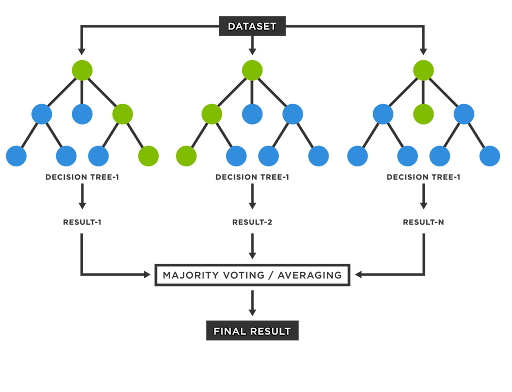
\includegraphics[width=0.5\linewidth]{contents/figures/LR RF diagram.jpg}
    \caption{Random Forest Visualisation \citep{verma_2022}}
    \label{fig:LR RF diagram}
\end{figure}

Training a RF model involves separating the dataset into subsets, and training multiple decision trees on each randomly assigned data subsetm as can be seen in figure \ref{fig:LR RF diagram}. After training, any test data, such as an image of a river and crops, is processed through all the decision trees, each voting on the class, with the average vote determining the final class. 

\begin{itemize}
    \item \textbf{Advantages:}
    \begin{itemize}
        \item Supported by PyCaret and scikit-learn libraries.
        \item The algorithm is logical and well-understood, making it intuitive. 
    \end{itemize}
    \item \textbf{Disadvantages:}
    \begin{itemize}
        \item Required involvement in model development means that this approach is still difficult to manually implement. 
    \end{itemize}
\end{itemize}

\subsubsection{Keras Sequential Model}
More recently, deep learning frameworks such as Keras have enabled the deployment of convolutional neural networks, often built using a simple Sequential model structure, that automatically learn hierarchical feature representations, offering state-of-the-art performance in high-resolution water body extraction challenges. 

Keras models, particularly the sequential model, are known for being one of the simplest ways of training neural networks with TensorFlow \citep{keras-team_2015} and PyTorch \citep{pytorch_2023}. The Keras Sequential model has been used in a TensorFlow tutorial demonstrating capability to classify different images of flowers. The dataset was over over 3,500 images \citep{tensorflow_2018} and after personally testing and adjusting the initially non-functional script to run locally instead of on Google Colab, the model was capable of achieving training data accuracy above 90\% running for 15 epochs. Theoretically, to create another image classification model for a different, bespoke purpose, such as reservoir classification, one would simply have to replace the training and test data used in this tutorial with the training data of their own application. 

\begin{itemize}
    \item \textbf{Advantages:}
    \begin{itemize}
        \item Straightforward implementation.
        \item Step-by-step, pre-made framework outlines all the important steps of model training, simplifying development. 
        \item Highly performant and well suited to image classification. 
    \end{itemize}
    \item \textbf{Disadvantages:}
    \begin{itemize}
        \item Black-box, more difficult to troubleshoot. 
    \end{itemize}
\end{itemize}

\begin{tabular}{@{}l p{0.35\textwidth} p{0.35\textwidth}@{}} 
\toprule
\textbf{Model} & \textbf{Keras Sequential} & \textbf{Random Forest} \\
\midrule
Model Type & Neural Network & Tree-based \\
Structure & Linear stack of layers & Decision Trees \\
Learning & Gradient Descent & Building Trees \\
Feature Learning & Often learns automatically & Uses provided features \\
Interpretability & Lower ("Black Box") & Higher (Feature Importance) \\
Typical Data & Images, Complex Patterns & Tabular, Structured Data \\
Common Library & Keras, TensorFlow & Scikit-learn, PyCaret \\
Core Idea & Hierarchical feature extraction and transformation & Averaging predictions of many diverse trees \\
\bottomrule
\end{tabular}

\subsection{Deep Learning}
Deep learning is a branch of machine learning that trains artificial neural networks with many successive layers to automatically learn large quantities of hierarchical representations of data \citep{nsoft_vision_2023}. Neural networks are named like this because they attempt to simulate the behaviour of the human brain. In a deep neural network, each layer transforms its input (for example, pixel values) into increasingly abstract features (edges, shapes, objects), which is the unique feature of deep neural networks that allow the system to perform complex tasks, such as image recognition from raw inputs. These changes can crucially be made without the programmer strictly coding this behaviour into the model \citep{holdsworth_scapicchio_2024}. 

At its core, a deep learning model consists of multiple “hidden” layers of interconnected "neurons". During training, the network adjusts millions of internal parameters to minimise prediction error on a labelled dataset. Modern architectures, such as convolutional networks for image recognition, build on this principle, enabling breakthroughs higher accuracies for predicting classes \citep{goodfellow_bengio_courville_2016}. These technologies have broader effects in many industries, such as the medical industry to identify tumors \citep{oróstica_mardones_bernal_molina_orchard_verdugo_carvajalhausdorf_marcelain_contreras_armisen_2025}, biological sciences for monitoring growth in organisms, autonomous driving \citep{barla_2021}, and the widespread use of artificial intelligence that operates on similar principles. 

\section{Machine Learning and Classification of Water Bodies}
Machine learning techniques have further enhanced water classification by learning complex spectral and spatial patterns directly from data \citep{ibm_2021b}. The integration of the various different approaches into remote sensing workflows, along with the increased availability of high-resolution satellite imagery has enabled more nuanced discrimination of water features such as "accurate water depth estimation" \citep{liu_wu_wu_zhou_2024} and improved adaptability to varying environmental conditions \citep{rahat_steissberg_etal_2023}.

There has also been research conducted in satellite imagery models being developed specifically for the classification of water reservoirs \citep{ghansah_2022_monitoring}, where the adopted approach was to implement a RF algorithm with no cloud masking required due to low cloud cover. Additionally, given that there is no mention of any spectral indices used for the detection of water, it is implied that the RF model was capable of extracting enough useful information from either a True Colour Image (TCI) or a Red-Green-Blue (RGB) composite to be trained adequately. This means that it appears that spectral indices were not required for effective water detection in Ghana's Upper-East region.

One of the main challenges associated with the study and classification of reservoirs, specifically in east England, is that it can be difficult to properly distinguish between reservoirs and irrigated cropland, waterlogged land, or even trees, as they reflect similar amounts of light in the relevant wavelengths. The approach of omitting the use of spectral water detection indices altogether adopted by \cite{ghansah_2022_monitoring} is one that may be more difficult to implement in this study due to these challenges. 

\subsection{Knowledge Gap}
Despite extensive work on water-index thresholds, machine learning classification, cloud masking, and large-scale water body mapping, no study to date has:
\begin{itemize}
    \item Validated model performance at 10\,m resolution over East England, where vegetation, soil moisture, and irrigation ditches introduce high false-alarm risk due to it being a heavily farmed region.
    \item Integrated end-to-end pipelines (cloud mask $\rightarrow$ water detection $\rightarrow$ classifier) into a single, reproducible workflow and assessed its generalisability across Sentinel-2 revisit cycles under varying seasonal conditions.
\end{itemize}

As a result, it remains unclear which combination of preprocessing and classifier yields robust detection of small agricultural reservoirs at 10m resolution, and how well such a pipeline can scale to routine monitoring for regional water-management agencies. Additionally, there is the informational knowledge gap of there simply not being an accurate register of the number of small reservoirs in the UK. 

Addressing this gap is the central objective of this thesis.

\chapter{Methodology}


\section{Overview}
This chapter will go through a detailed explanation of each step that should be taken to replicate this software developed for this thesis, starting from nothing more than a Python interpreter. It is important to note that the vast majority of the software development for this project (every change from February onwards) has been documented and explained with comments, descriptions, and a \verb|readme.md| file on a publicly accessible GitHub repository named IPDMP. The link to the Individual Project Data-to-Model Pipeline (IPDMP) repository, as well as an extensive "code walk-through" for each major program discussed can be found in Appendix B. 

\subsection{Section Description}
The methodology for this thesis fundamentally consists of four key steps, which align with the objectives defined in the introduction section. This is a brief overview of the upcoming sections covering brief objective. 
\subsubsection{Objective 1: Image Selection}
\begin{itemize}
    \item Select one appropriate satellite image for the development of the necessary software tools and three more satellite images for model deployment. 
\end{itemize}
The first step is to conduct image download. The two approaches for this application are to either download images locally or use a web-based database such as Google Earth Engine. For this study, locally downloading data is appropriate because there is no need to scale up to a large time period or study area yet. 

\subsubsection{Objective 2: Data Generation}
\begin{itemize}
    \item Develop a software tool to automate satellite imagery handling/pre-processing and facilitate the semi-automated creation of labelled training data through a dedicated user interface. 
\end{itemize}
NALIRA, a Python program, automates the generation of training data from Sentinel 2 imagery, avoiding manual labelling. It processes satellite images by extracting bands, performing cloud masking, calculating indices, and optionally displaying plots. The True Colour Image and index plots are divided into user-defined chunks to simplify labelling. Users are prompted to input the number of reservoirs and water bodies per chunk. If present, a GUI enables users to label these features as Regions of Interest (ROIs), with coordinates saved in a CSV file that undergoes rigorous automated validation. This chunk-wise approach allows for breaks and revisiting previous labels. Finally, the labelled coordinates are used to extract individual reservoir/water body images (and corresponding non-water land images) for training data, sized at $\frac{1}{25}$ of the original chunk.

\subsubsection{Objective 3: Model Training}
\begin{itemize}
    \item Build, train, and validate a machine learning classification model (specifically using the Keras Sequential model) for water reservoirs, non-reservoir water bodies, and land.
\end{itemize}
The third step is to train the machine learning model that will identify reservoirs, water bodies, and land. This is done using a repurposed Google Colab TensorFlow tutorial initially intended for flower classification with a Keras Sequential Model !!! CITE THIS CITE THIS CITE THIS !!!. To repurpose this tutorial, several unnecessary, non-functional, or superfluous steps were removed, reliability was improved by adding robustness to the process, and the original flower classification training data was swapped out for the images generated with NALIRA. The program encompassing the deployment of the model is called the Keras Reservoir Identification Sequencing Platform, abbreviated to KRISP. The program dedicated to the training and initial validation of the final model is called KRISP Trainer. 

\subsubsection{Objective 4: Model Deployment}
\begin{itemize}
    \item Deploy the model over East England and produce a map of the quantity, location, and size of all water reservoirs in East England for March 2025. 
\end{itemize}
The fourth and final step is to deploy the model. For this, the program created is the aforementioned KRISP program. This Python script ingests an un-processed and unseen satellite image from Sentinel 2 then conducts very similar initial steps to NALIRA (image manipulation, cloud masking, index calculation, optional display of the index calculated, optional TCI manipulation, and separation of the full-sized image into chunks smaller chunks). After these steps are complete, KRISP further separates each chunk into 25 "mini-chunks" to match the size of each box containing a training image. This is done to ensure that the test and deployment data for KRISP is the same dimensions as the test upon which KRISP was trained, maximising accuracy and minimising error. 

\section{Objective 1: Image Selection}
\subsection{Satellite Choice}
The satellite of choice for this thesis is Sentinel 2 because of the higher resolution options compared to Landsat 7-9. Additionally, for low-computation troubleshooting, the Sentinel 2 image folders also have a 60m resolution option, reducing time spent on opening and handling the otherwise larger image arrays. 

\subsection{Satellite Compatibility}
While the KRISP trainer program was developed primarily with Sentinel 2 in mind, it is entirely sensor-agnostic, meaning that dependent on specifically Sentinel 2 data. The KRISP trainer program is not only sensor-agnostic, but also 

The NALIRA program was initially developed for Landsat 7 images, then it was adapted for compatibility with any processing level of Landsat 8 and 9 as well. Then, Sentinel 2 data was introduced, and there was a brief period where NALIRA was capable of accepting any image from Landsat 7, Landsat 8, Landsat 9, Sentinel 2A, Sentinel 2B, and Sentinel 2C. 

\subsection{Image Download}
To download images for Sentinel 2, the Copernicus browser must be used. To access these files it is necessary to log in or create an account, which can be done easily by registering a valid email address. 
\begin{figure}[H]
    \centering
    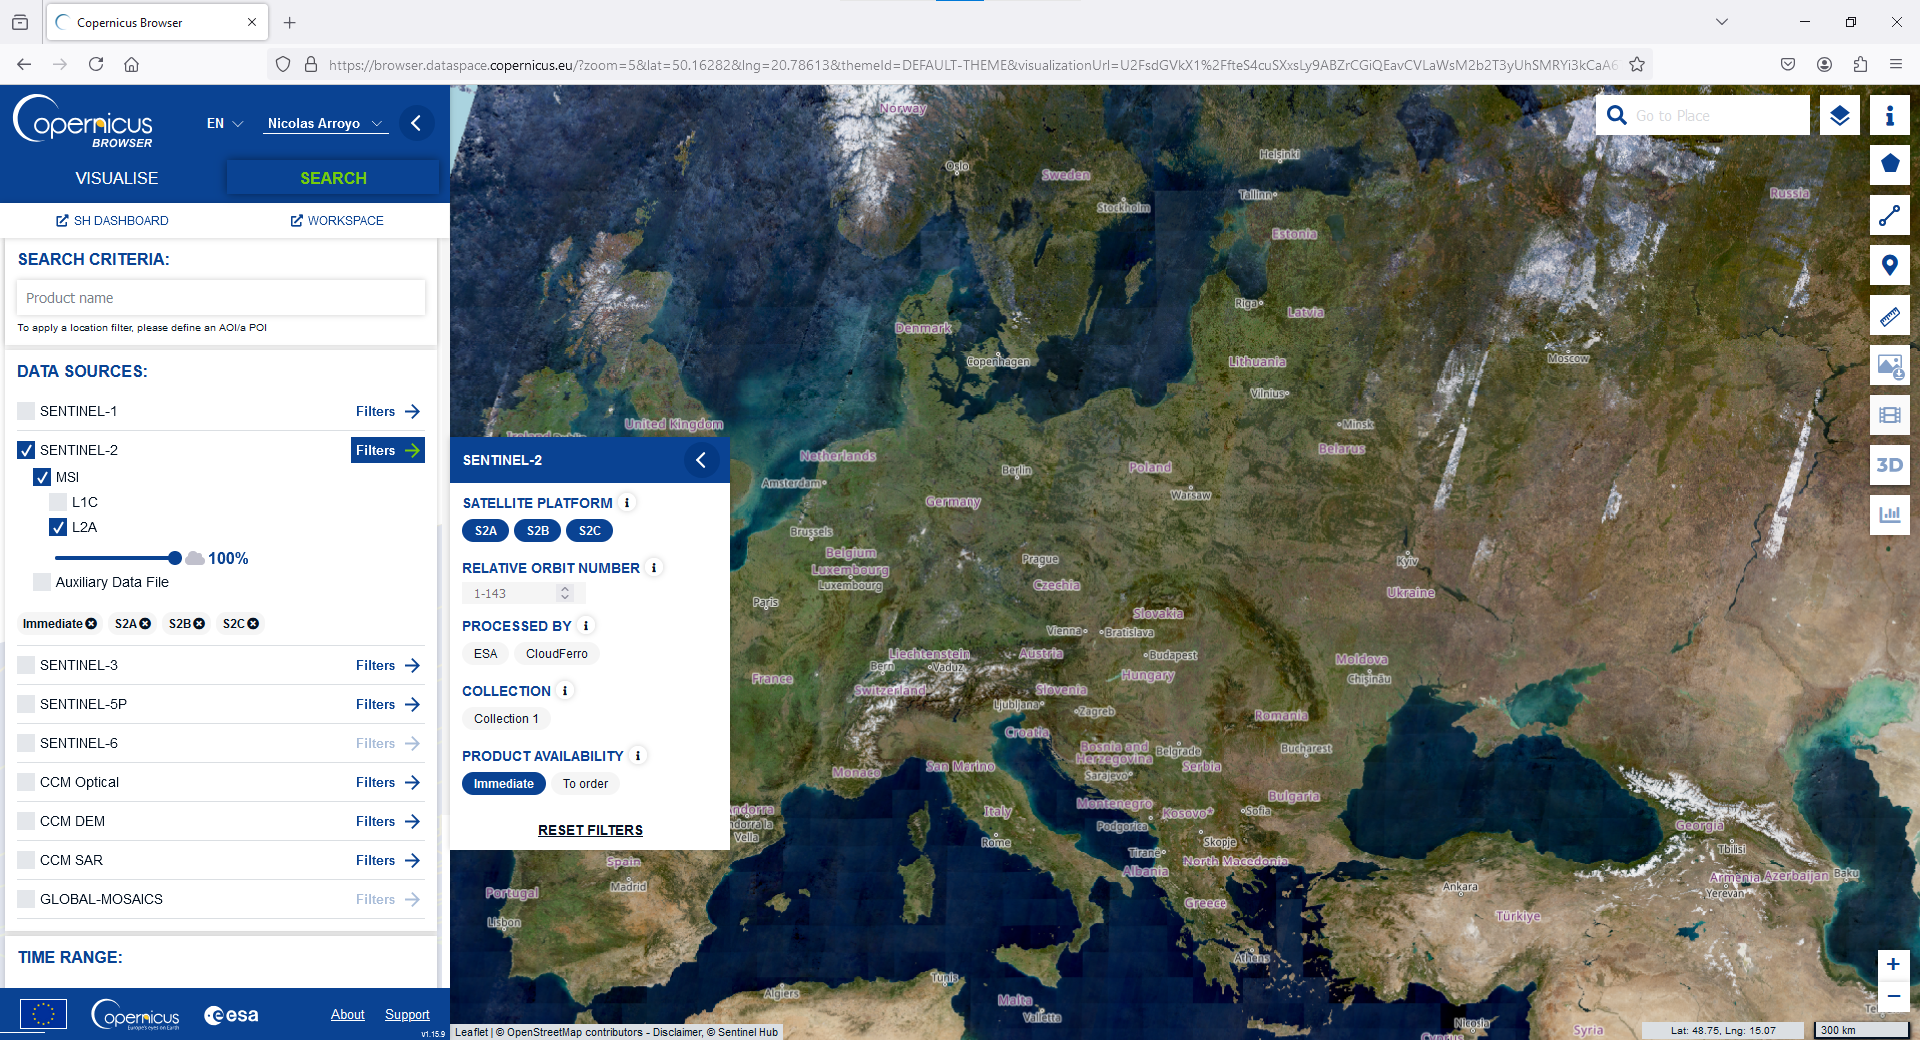
\includegraphics[width=0.5\linewidth]{contents/figures/ME copernicus detailed search.jpg}
    \caption{Copernicus browser detailed search}
    \label{fig:ME copernicus detailed search}
\end{figure}
After logging in or registering an account, the first step of downloading images is to select the appropriate satellite. This thesis focuses on Sentinel 2 images, so we must filter out all other satellites that would not be compatible (figure \ref{fig:ME copernicus detailed search}. Go to "SEARCH" on the upper left and select "SENTINEL 2" $\rightarrow$ "MSI", which stands for Multi-Spectral Instrument. Then, select only "L2A" to filter down the images to the second processing level offered by Sentinel 2. After this, select "Filters" and choose S2A, S2B, and S2C platforms to allow for images from any of the three satellites in the Sentinel constellation.

\begin{figure}[H]
    \centering
    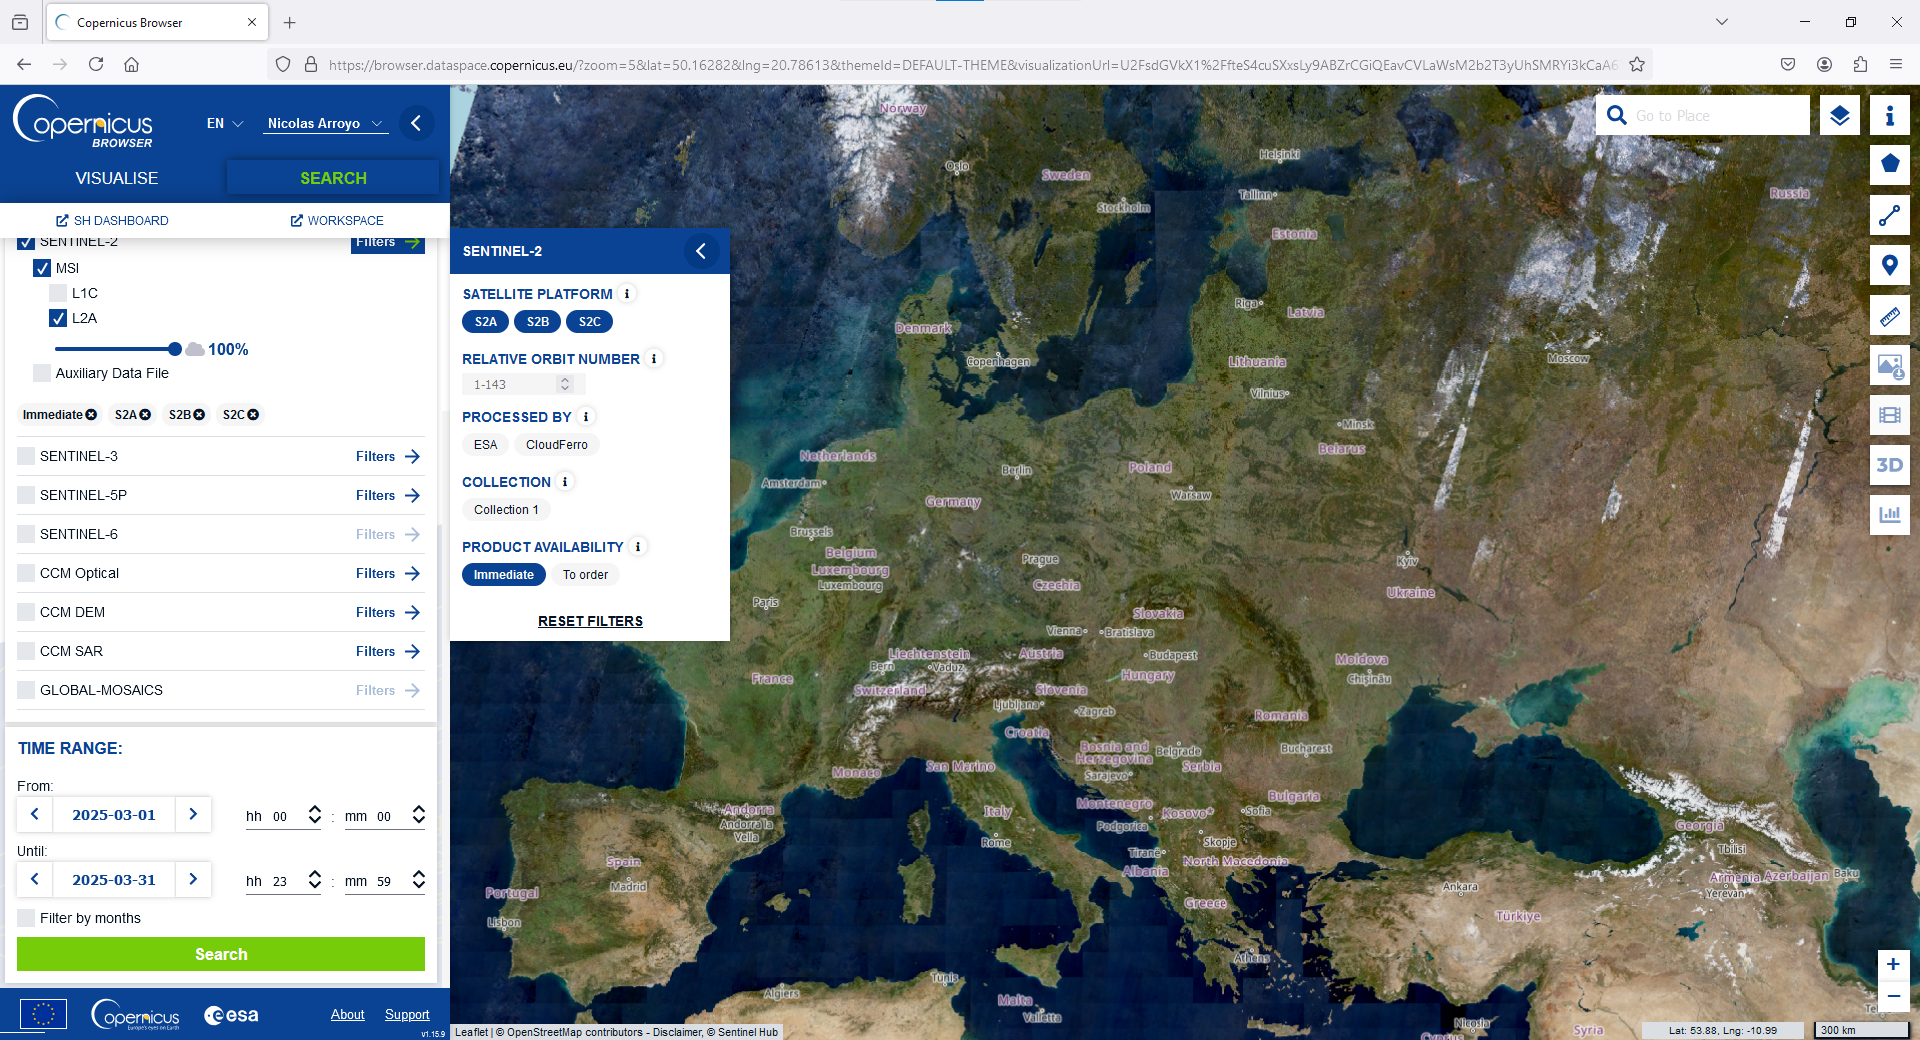
\includegraphics[width=0.5\linewidth]{contents/figures/ME copernicus time range.jpg}
    \caption{Copernicus browser time range example}
    \label{fig:ME copernicus time range}
\end{figure}
Once the satellite platform has been selected, scroll down on the sidebar to reach the time frame of the image (figure \ref{fig:ME copernicus time range}. The time period for this study is the month of March 2025, as was discussed in the introduction, so select "2025-03-01" in the "From:" field and "2025-03-31" in the "Until:" field to encompass this period. Once both time period and satellite platform have been defined, press the green "Search" button at the bottom. 

\begin{figure}[H]
    \centering
    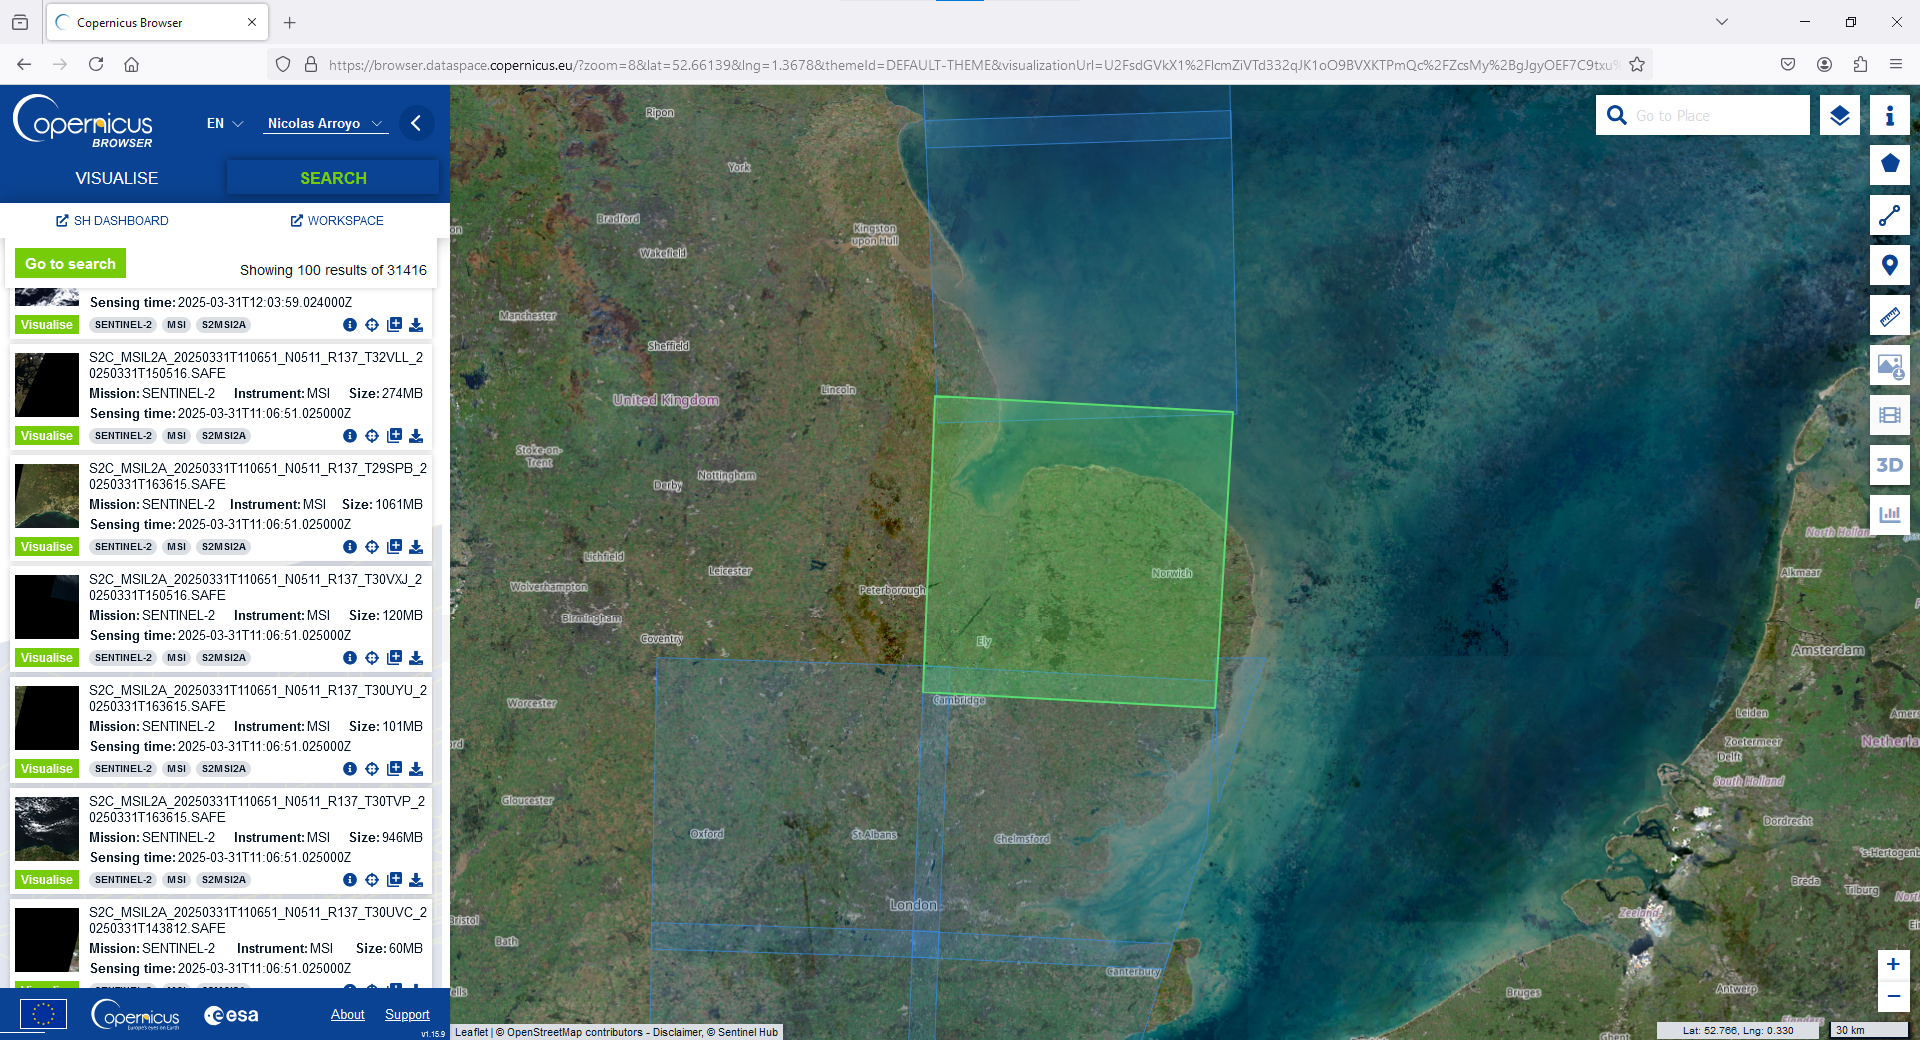
\includegraphics[width=0.5\linewidth]{contents/figures/ME copernicus example chunk.jpg}
    \caption{Copernicus browser image example}
    \label{fig:ME copernicus image example}
\end{figure}
The Copernicus browser will take some time to load the images. After you can see the image names on the left-hand side of the screen, select one where the land is clearly visible in the East Midlands area, as demonstrated in figure \ref{fig:ME copernicus image example}. To download this image, simply press the download button as demonstrated in figure \ref{fig:ME copernicus download example} and wait for the file to download completely. Note: satellite image files are usually very large (around 1 GB in size). The files are packaged in \verb|.zip| folders on Windows which have to be extracted. Further image processing and data generation will increase the required storage available, so ensure you have at least 5 GB available on disk, or use online storage solutions. This is discouraged as there have been incidents of files being deleted automatically by services like OneDrive. 

\begin{figure}[H]
    \centering
    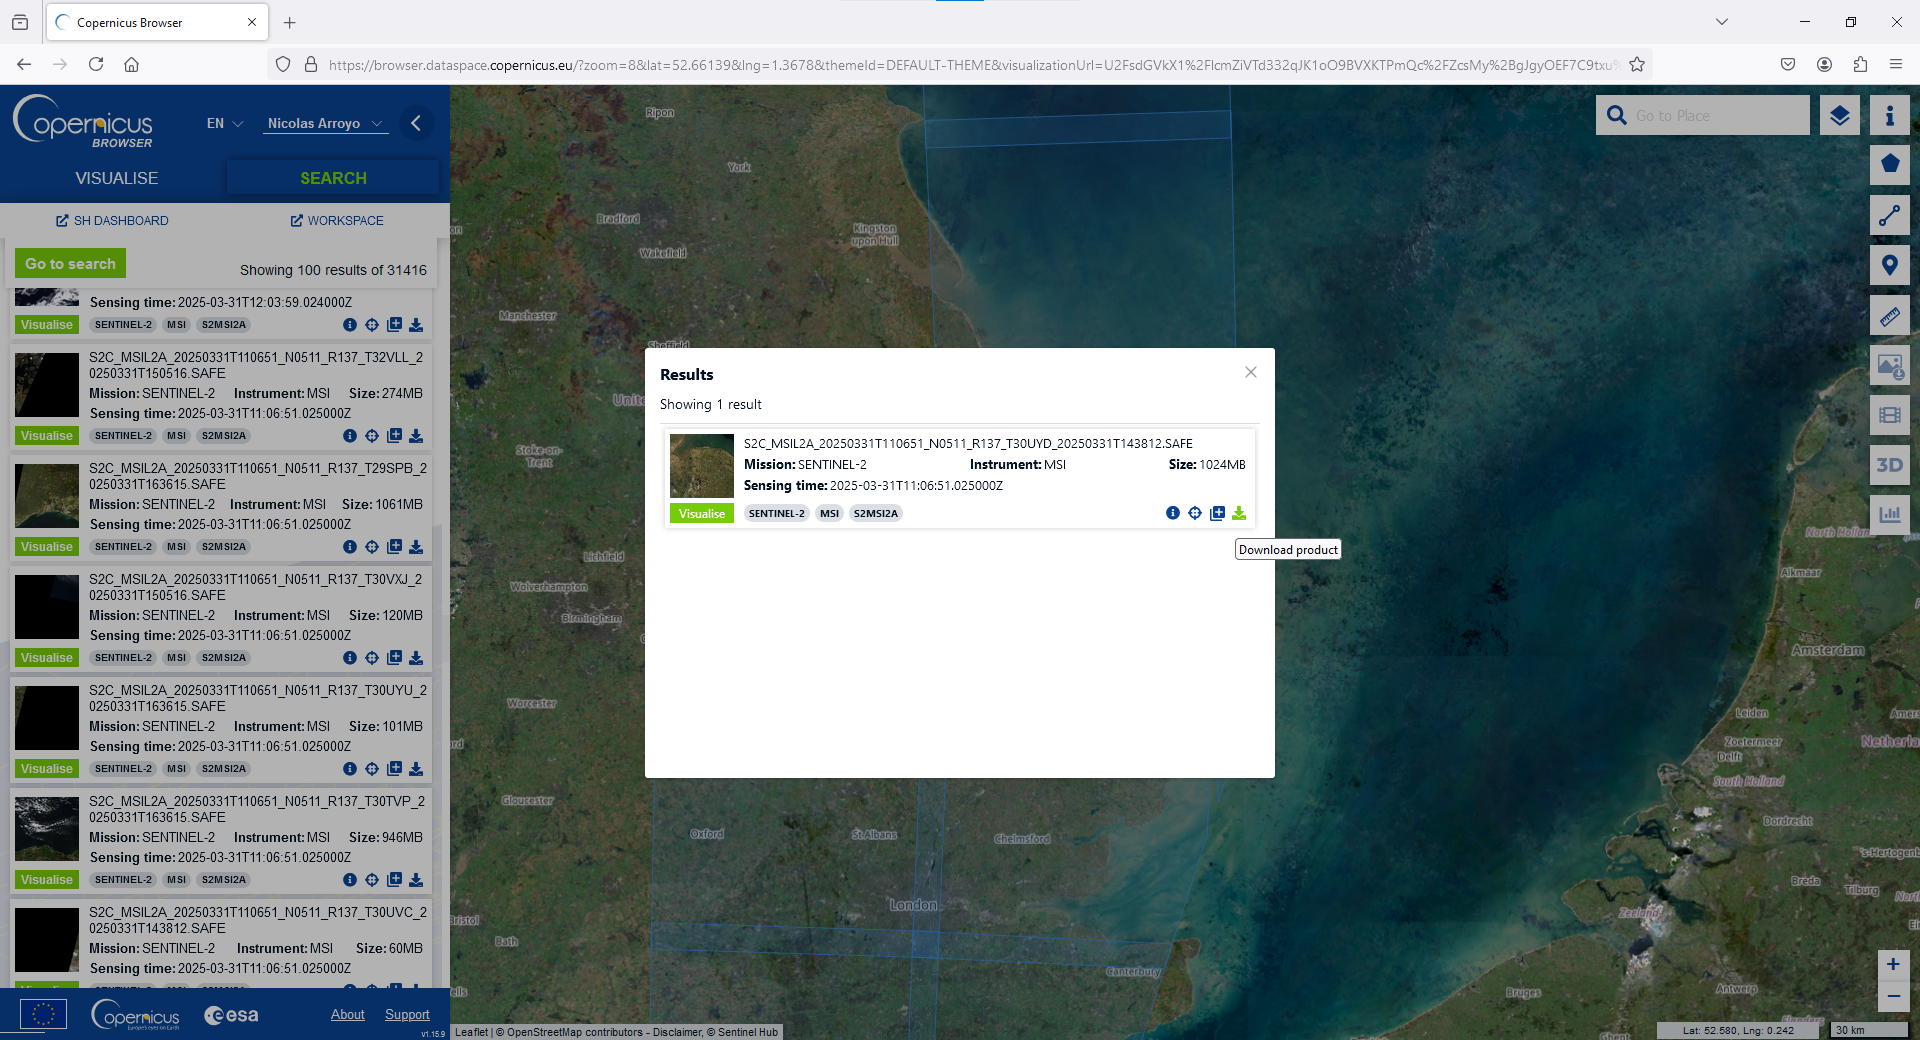
\includegraphics[width=0.5\linewidth]{contents/figures/ME copernicus download example.jpg}
    \caption{Copernicus browser download example}
    \label{fig:ME copernicus download example}
\end{figure}
Once the image folder has downloaded completely, extract the zip file to a known location, preferably close to the root of your drive to prevent \verb|maximum path length| errors. This error occurs when Python or the operating system tries to access a file but the path to that file is too long (above 250 characters). This can be disabled when installing Python, but to avoid any potential problems, it is generally good practice and strongly recommended to store this folder close to the root. 

For example:

"\verb|C:\Users\abcde\Sen2|" 

as opposed to something like 

"\verb|C:\Users\abcde\Documents\Satellite Image Downloads\Sentinel 2|"

\begin{figure}[H]
    \centering
    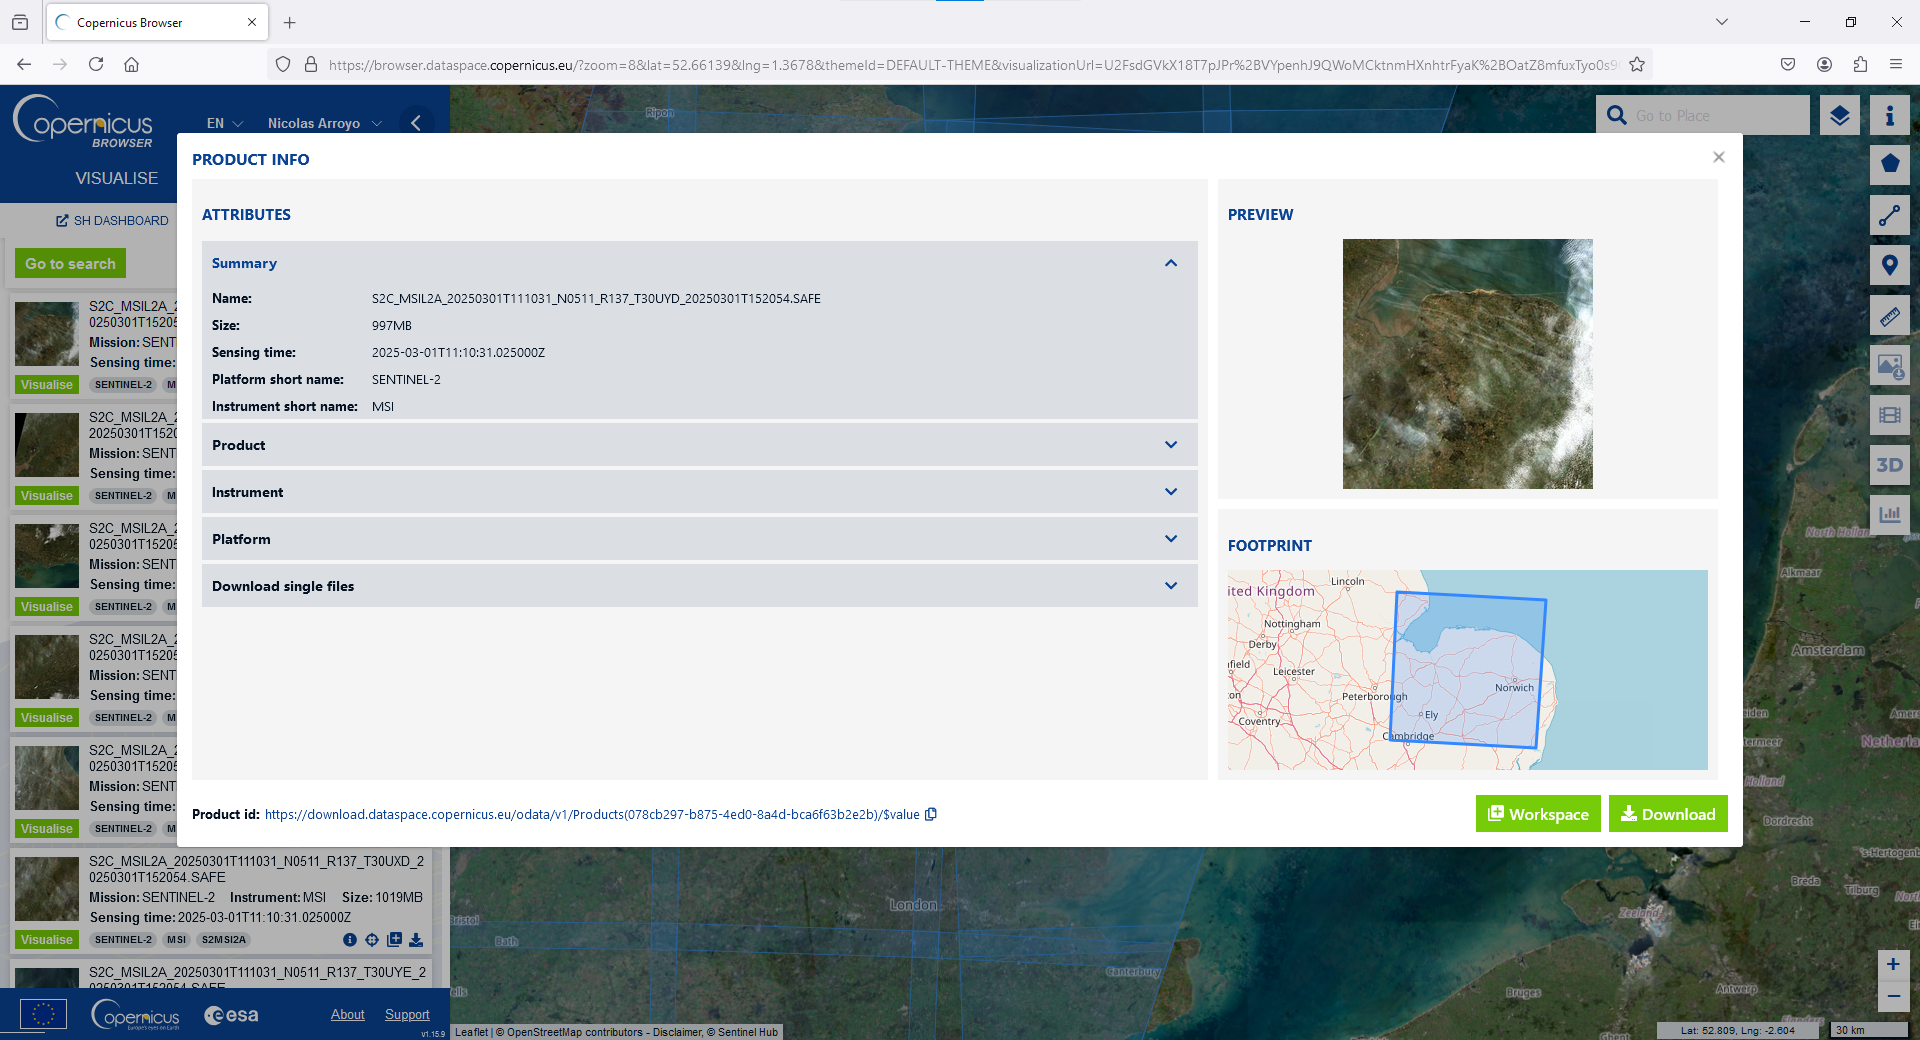
\includegraphics[width=0.5\linewidth]{contents/figures/ME copernicus exact chunk.jpg}
    \caption{Copernicus browser exact development image used}
    \label{fig:ME copernicus exact image}
\end{figure}
The actual image used for initial program development is the one shown in figure \ref{fig:ME copernicus exact image}. The name of this image is as follows: 

\verb|S2C_MSIL2A_20250301T111031_N0511_R137_T31UCU_20250301T152054.SAFE|

For all following file naming explanation or referencing, this is the image name that is being used. 

\subsection{Sentinel File Naming Convention}
Each satellite image folder from the Sentinel satellites follows the same naming convention. This simplifies file searching and enables the automation developed with NALIRA. All the main, important details about a given satellite image is stored in its folder name, and anything that is seen as too granular to include in the name is stored in various meta-data files within the folder. For this study, none of the meta-data information is necessary, so it is important to first explain the meaning of the image folder name. 

Every section of information is split up with underscores ("\verb|_|"), so in total there are seven main sections. We will use the exact image folder that was used for program development in this study to identify these sections. All of this information is given by \cite{copernicus_2025}

\verb|S2C_MSIL2A_20250301T111031_N0511_R137_T31UCU_20250301T152054.SAFE|

\subsubsection{S2C}
The first section is simply the name of the satellite. In this case, "S2C" stands for "Sentinel 2 C". This bit could also be "S2A" or "S2B" if using Sentinel 2 A or Sentinel 2 B. 

\subsubsection{MSIL2A}
This sections contains two pieces of information: the first three characters, "MSI" are the abbreviation of the instrument used (MSI = Multi-Spectral Instrument) and the last three characters are the product level (L2A = Product Level 2, meaning that some post-processing has been applied). 

\subsubsection{20250301T111031}
This is the "datatake start sensing" time. It is split up into the format: 

\verb|YYYYMMDDTHHMMSS|, where \verb|YYYYMMDD| is the year, month, and day, and \verb|HHMMSS| is the hour, minute, and second of the day that the sensor started imaging to produce this data. The \verb|T| character is used to separate the data and time. 

\subsubsection{N0511}
This is the "Processing Baseline Number", which gives more information about the processing level. 

\subsubsection{R137}
This is the "Relative Orbit Number", which can range from \verb|001| to \verb|143| because 143 is the number of full orbits that the satellites make before completing a full cycle. 

\subsubsection{T31UCU}
This is the "tile number field", which essentially describes the 110 km x 110 km area being imaged. There are enough tiles to cover everywhere that a Sentinel 2 satellite could take an image of, so we can use this section to find where on Earth the image is covering. This information can then be used to conduct image compositing, which, although not implemented for this project, is a possible area of future development. 

\subsubsection{20250301T152054.SAFE}
Finally, this section is the "Product Discriminator". It follows the same format as the datatake start sensing time, however it can be slightly earlier or later than the start time depending on which product it is describing. 

The \verb|.SAFE| suffix is the "Standard Archive Format for Europe". 

\subsubsection{Sub-folders and files}
The image sub-folder contained in the main image folder may have a different format to each other, however, the sub-folder is always the only item in that level of the directory, so it is relatively simple to search the level and find the sub-folder. The image files themselves all follow a cohesive format. 

If we are trying to access a \verb|10m| resolution \verb|green| band image, we first need to recall which band on Sentinel 2 senses the green wavelength. In table \ref{tab:LR s2 band wavelengths and resolutions}, we can see that the green band is number \verb|3|. We can combine the tile number field, the datatake start sensing time, the band number, preceded by the letter \verb|B| and a \verb|0| if it is a single digit band number, and the resolution. At the end, we have to place the image file format, which is \verb|JPEG2000| for Sentinel 2 images. This is a lossless version of the \verb|jpg| format, and it means that all images are stored with the \verb|.jp2| file extension. The native Windows photo viewer is not capable of opening these images, so it may be helpful to install an image manipulation program like \verb|GIMP| to view these images, although it is not necessary for the processes outlined here. This yields the following file name: 

\verb|T31UCU_20250301T111031_B03_10m.jp2|

This image file is stored within subdirectories of the main folder, and this will be covered in an upcoming section. 

\section{IPDMP System Overview}
The Individual Project Data-to-Model Pipeline (IPDMP) comprises three core Python scripts designed for the classification of small water reservoirs using Sentinel 2 satellite imagery. The overall process involves data generation and labelling (NALIRA), model training (KRISP trainer), and model deployment for prediction (KRISP).

For this study, the Normalised Difference Water Index (NDWI) is selected as the primary spectral index for data labelling and model training/validation due to its ability to leverage Sentinel-2's high-resolution bands (Green and NIR). While other indices like MNDWI, AWEI-SH, and AWEI-NSH are calculated in NALIRA to aid manual labelling by providing multiple visual inputs, the machine learning model focuses on NDWI-derived data.

\begin{lstlisting}[language=Python, caption=Calculation of Water Detection Indices]
np.seterr(divide="ignore", invalid="ignore")
ndwi = ((green - nir) / (green + nir))
mndwi = ((green - swir1) / (green + swir1))
awei_sh = (green + 2.5 * blue - 1.5 * (nir + swir1) - 0.25 * swir2)
awei_nsh = (4 * (green - swir1) - (0.25 * nir + 2.75 * swir2))
\end{lstlisting}

Cloud masking employs a basic numerical threshold approach. Pixels in the Sentinel-2 cloud probability band (\verb|MSK_CLDPRB|) with a likelihood greater than 50\% are masked (set to NaN or zero) in the band images before index calculation. This simple method is deemed sufficient due to the selection of imagery from a period with known low cloud cover (March 2025). For applications in cloudier periods, more advanced masking techniques (e.g., FMask) and image compositing would be necessary.

A custom Keras-based Convolutional Neural Network (CNN) model, adapted from a TensorFlow tutorial, is used for classification. This approach offers flexibility and aims for good generalisation on the study area. The model is trained to classify image segments into 'reservoirs', 'water bodies' (non-reservoir), or 'land'. The KRISP script then deploys this trained model, applying it iteratively across small image chunks ('mini-chunks') derived from the larger satellite scene, effectively acting as an object detection mechanism for water reservoirs.

\subsection{Helper Functions}
To improve code readability, each of the programs discussed below make use of helper functions. This also improves the efficiency of the code as fewer variables need to be stored in memory and each file is itself smaller

\section{Objective 2: Data Generation (NALIRA)}
The second step is to generate training data. Rather than lengthy and laborious manual labelling, this study develops the Navigable Automated Labelling Interface for Regions of Attention, abbreviated to NALIRA. 

This Python program ingests a Sentinel 2 satellite image, extracts the necessary bands for index calculation, conducts cloud masking, performs index calculations, optionally displays the plots of the indices calculated, manipulates a "True Colour Image" (TCI) found in the Sentinel 2 data folder, and separates the images and index plots into a user-defined number of "chunks". This is done to make data labelling easier for the user as it allows them to split the process up into shorter period of data labelling. So far, the entire process described is entirely automated to offload user intervention onto robust checks and verifications done automatically by the program. 

After the images are split into chunks, the user is iteratively prompted with each chunk and they must enter the number of reservoirs and water bodies in the chunk. If they input one or more of either class, a Graphical User Interface (GUI) is produced for the user to identify (label) those reservoirs or water bodies which are named and saved as regions of interest (ROIs). These "chunk-wise" coordinates are saved to a "comma-separated values" (CSV) format file. 

This file is rigorously checked for file and data validity before the data labelling process even begins, and if any error or inconsistency is found, the user is prompted to fix the error before being allowed to proceed. The file is also checked continuously with every successive chunk to ensure minimal chance of failure, which could result in the loss of a large amount of training data. 

During data labelling, the user is also able to take a break and the progress is automatically saved on disk, or return to any previous chunk examined to view it again and overwrite their entry, introducing the navigable element of NALIRA. Once data labelling is either complete for the entire image or the user has decided to take a break, the automation is resumed and the chunk-wise coordinates are used to individually isolate each reservoir and water body in an image $\frac{1}{25}$ the size of the chunk and that image is saved as training data for both NDWI and TCI. Similar images are saved for non-water land by selecting the top left corner of each chunk with no reservoir or water body. 

\subsection{NALIRA Code Walk-through}


\section{Objective 3: Model Training (KRISP Trainer)}
This script trains the Keras CNN model using the segmented image data generated by NALIRA. This is the script that was adapted from an existing image classification tutorial created to classify images of different types of flowers \citep{imageclassification_2024}. 

\subsection{Changes from Flower Classification}
Originally, the flower classification tutorial had several steps which were not directly applicable to this study, as can be seen in figure \ref{fig:ME outline OG flower classification}. 

\begin{figure}
    \centering
    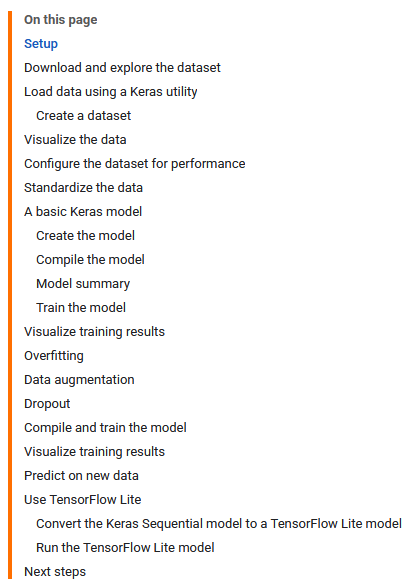
\includegraphics[width=0.5\linewidth]{contents/figures/ME outline of flower classification.jpg}
    \caption{Table of Contents for the original flower classification tutorial \citep{imageclassification_2024}}
    \label{fig:ME outline OG flower classification}
\end{figure}

Some of the steps up to \verb|A basic Keras Model| are necessary for proper data handling, although they had to be adapted to function with the specific paths used in KRISP Trainer. Most of these initial steps, however, are not necessary for the function of KRISP Trainer, such as \verb|Visualize the data| which simply chooses an image from the dataset and displays it in the console. These steps were removed for KRISP Trainer, which is solely concerned with handling data and training the model. 

The basic Keras model created in the tutorial is used as a way of showing the common pitfalls of machine learning, specifically overfitting, and the two techniques used to mitigate this problem, data augmentation and dropout. To avoid training unnecessary models, the training of the basic Keras model with no mitigations against overfitting was removed altogether, but the strategies of data augmentation and dropout were both included in the training of the final model. 

The steps of \verb|Compile and train the model|, \verb|Visualize training results|, and \verb|Predict on new data|, were all preserved and adjusted for KRISP Trainer. Although visualising training results is not explicitly necessary for model training, it is helpful for identifying the ideal duration of training and for spotting the inflection point as the model suffers from overfitting. 

\begin{figure}
    \centering
    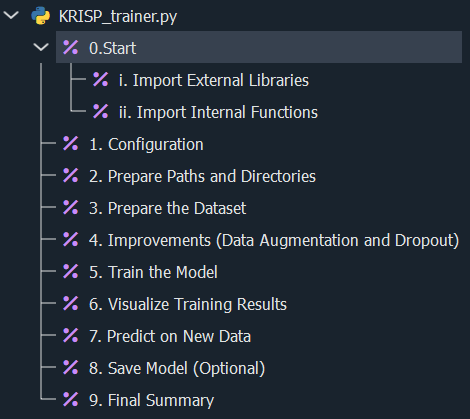
\includegraphics[width=0.5\linewidth]{contents/figures/ME KRISP trainer outline.jpg}
    \caption{Table of Contents for KRISP Trainer \citep{imageclassification_2024}}
    \label{fig:ME outline krisp trainer}
\end{figure}

As can be seen from figure \ref{fig:ME outline krisp trainer}, the contents of KRISP Trainer are significantly reduced to the ones of the original flower image classification tutorial. Given that the tutorial is designed to explain each step in detail, the steps that were deemed "unnecessary" are in reality very useful in understanding the strategies behind the training of a Keras model. However, efficiency and performance are a priority throughout this project, so KRISP Trainer keeps only the essentials from the flower classification tutorial and the rest is reworked for the purposes of this particular study. 

\subsection{KRISP Trainer Code Walk-through}


\section{Objective 4: Model Deployment (KRISP)}
This script deploys the trained Keras model (saved by \verb|KRISP_trainer|) to classify mini-chunks generated from a larger Sentinel-2 scene. While the KRISP program makes predictions over a given number of chunks, the KRISP-Yield program (KRISP-Y) was developed to yield the data (predictions) made by KRISP and to save everything to a CSV file. 

\subsection{KRISP Code Walk-through}

\subsection{KRISP-Y Code Walk-through}

\section{Technical Challenges}
\subsubsection{Identifying water}
One of the main challenges in this research will be the differentiation between water reservoirs from land areas, or other bodies of water. Below is a screenshot taken from Google Maps showing a farm in east England with a water reservoir in the middle, some tree cover nearby, and a house. 

\begin{figure}[H]
\centering
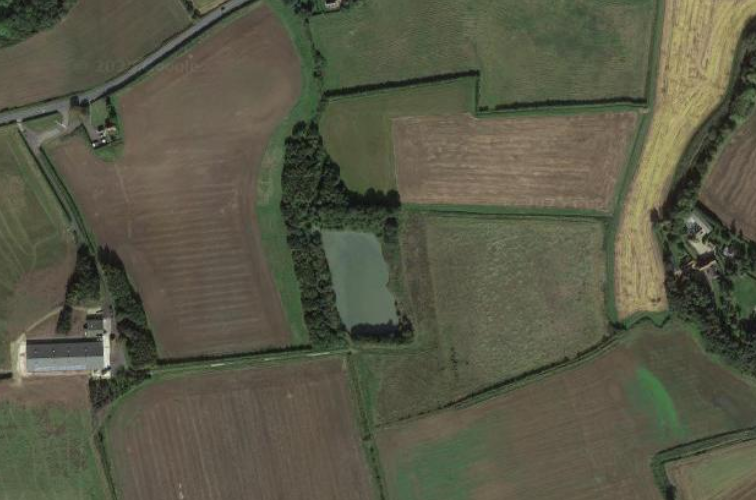
\includegraphics[width=0.4\textwidth]{contents/figures/gmaps screenshot.jpg}
\caption{Google Maps screenshot showing a water reservoir near trees}
\label{fig:NISH}
\end{figure}

In this example, a human could easily identify that the upper right side of this image shows trees, and the lower left side shows a river with a nearby water reservoir. However, a computer algorithm may find this differentiation more difficult, as relying solely on colours may lead it to the conclusion that both sides of the image contain a water reservoir. Instead, more complex techniques must be adopted that allow the computer to determine the shape, surrounding area, and other contextual information about the water reservoir. For this reason, one of the goals of this project is also to determine what the most valuable metrics are, from a satellite imagery perspective, for identifying water reservoirs. A further challenge will then be implementing these metrics and training a machine learning algorithm to make use of them to classify large areas of land. 

\subsubsection{Cloud Contamination}
Satellite imagery can come in many different levels of quality, and one of the main problems that have to be mitigated for is potential cloud cover. Clouds can partially or completely obscure important features on land or they can 'trick' a program into predicting a water feature instead of a cloud or the shadow of a cloud. As mentioned before, the time period for this study was specifically selected to avoid this problem entirely, however for the cases where clouds still cover part of the image, rudimentary cloud masking has been implemented, and will be discussed in further detail in upcoming sections. 

\subsubsection{Machine Learning Development}
There are also technical challenges that come with machine learning. Although resources for learning about this topic have improved in the past few years, there is still a steep learning gradient, particularly for one with little background in computer science. For this reason, the researcher has diligently documented progress on software development in this project with a public code repository which can be found linked in Appendix B. 

\section{Online Code Repository (GitHub)}
See appendix B


\chapter{Results}


\section{Objective 1: Image Selection}
\subsection{Landsat Development Images}

\subsection{Sentinel Development Image}

\subsection{Sentinel Deployment Images}

\subsection{Uncertainty Analysis}

\subsection{To what extent was the objective met?}


\section{Objective 2: Data Generation (NALIRA)}
\subsection{Main Features}
\subsubsection{Navigability}
\subsubsection{Scalability}
\subsubsection{Automation}
\subsubsection{Interface}
\subsubsection{Robustness}

\subsection{Uncertainty Analysis}

\subsection{To what extent was the objective met?}


\section{Objective 3: Model Training (KRISP Trainer)}
\subsection{}
\subsection{To what extent was the objective met?}

\section{Objective 4: Model Deployment (KRISP)}
\subsection{Accuracy}

\subsection{Precision}

\subsection{Uncertainty Analysis}

\subsection{To what extent was the objective met?}



\chapter{Discussion}


\section{Overview}
The overarching method employed is fundamentally a four-step process which aligns with the objectives defined in the introductory section. 

\subsection{NALIRA: Objectives 1 \& 2}
\subsubsection{}
\subsubsection{Implication on Aim and Objectives}

\subsection{KRISP Trainer: Objective 3}
\subsubsection{Implication on Aim and Objectives}

\subsection{KRISP: Objective 4}
\subsubsection{Implication on Aim and Objectives}


\section{Contextualisation Within the Field}


\section{Limitations}
\subsection{Cloud Masking Approach}
\subsubsection{Analysis of Impact on Results}

\subsection{Limited Training Data}
\subsubsection{Analysis of Impact on Results}

\subsection{Computational Power}
\begin{itemize}
    \item Satellite imagery is composed of several high-resolution images of a specific wavelength of light. 
    \item This means that each single "image", which in reality is packaged as a folder of images, contains many hundreds of megabytes (MBs), and sometimes over a gigabyte (GB) worth of data. 
    \item Handling this large quantity of data can be highly computationally intensive and slow if implemented incorrectly, therefore, in the explanation of the programs developed for this study, it should be noted that a majority of the time spent working on the code was to optimise and refine memory usages, Input/Output (IO) handlings, and various other efficiency improvements. 
\end{itemize}
\subsubsection{Analysis of Impact on Results}
Low



\chapter{Conclusion}


\section{Summary of Results}


\section{Areas of Future Work}
\subsection{General Knowledge Gaps}
\begin{itemize}
    \item quantify accuracy of OmniWaterMask
\end{itemize}

\subsection{Suggested Further Development}
\begin{itemize}
    \item NALIRA
    \begin{itemize}
        \item higher resolution satellite compatibility
        \item code efficiency optimisations (IO handling, multithreading, caching - could talk about CPU and GPU (they are in the nomenclature))
        \item proper index thresholds
        \item image compositing for adaptation to months with more cloud cover
        \item actual cloud masking
        \item switch to pandas from just writing all the damn data handling yourself you thick moron
    \end{itemize}
    \item KRISP and KRISP Trainer
    \begin{itemize}
        \item sensitivity analysis on optimal number of epochs
        \item image composites
    \end{itemize}
\end{itemize}

\section{Wider Applications}
\subsection{Environmental: Support Policy Decision-Making}
\begin{itemize}
    \item This research has the potential to inform water infrastructure LCA, aiding in the optimisation of resource management strategies. 
    \item It can also support the planning of renewable energy projects by providing reliable water data for cooling and thermal storage in low carbon heating networks. 
\end{itemize}
\subsection{Biology: Zebrafish Angiogenesis Study}
max

\appendix
\chapter{Project Management}
\section{Constraints From Other Unit Commitments}


\section{Reflection}
\subsection{Initial Plan}

\subsection{Updated Plan}

\subsection{Final Plan}

\subsection{Discussion on Plan Effectiveness}

\subsection{Impact on Future Projects}



\chapter{Code Link and IPDGS User Interface}
\section{Code}
github link: \url{https://github.com/nicoarrroyo/IPMLS/tree/main}

\section{IPDGS User Interface}
me when i'm an ipdgs user interface

\begin{figure}
     \centering
     \begin{subfigure}[b]{0.3\textwidth}
         \centering
         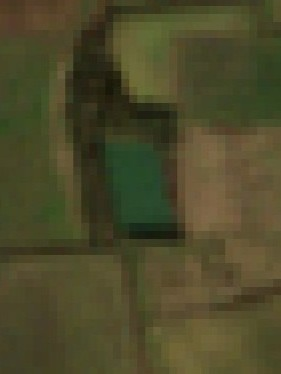
\includegraphics[width=\linewidth]{contents/figures/LR 10m res.jpg}
         \caption{User prompted on number of reservoirs}
         \label{fig:ipdgs ui first prompt}
     \end{subfigure}
     \hfill
     \begin{subfigure}[b]{0.3\textwidth}
         \centering
         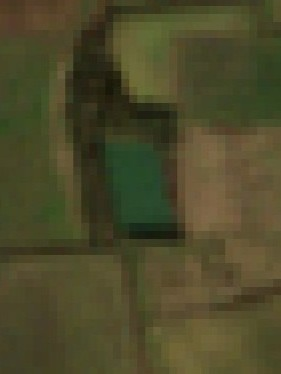
\includegraphics[width=\linewidth]{contents/figures/LR 10m res.jpg}
         \caption{User creating a polygon of the reservoirs' coordinates}
         \label{fig:ipdgs ui polygon}
     \end{subfigure}
     \hfill
     \begin{subfigure}[b]{0.3\textwidth}
         \centering
         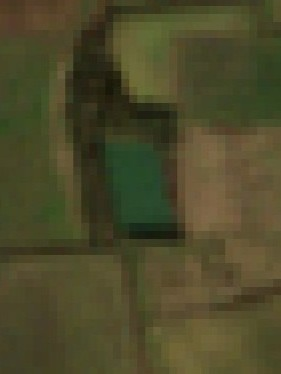
\includegraphics[width=\linewidth]{contents/figures/LR 10m res.jpg}
         \caption{IPDGS automatically generates the next chunk}
         \label{fig:ipdgs ui next chunk}
     \end{subfigure}
        \caption{Example IPDGS User Interface}
        \label{fig:ipdgs ui}
\end{figure}



\chapter{Supplementary Results}
\input{contents/apndx_c_supplementary_results}

\chapter{Additional Explanations}
\section{Technical Background}
Now I will provide some background information to the technical aspects of this study. This study involves the training and application of a machine learning model which uses satellite imagery as its input data and is implemented in the Python programming language. This subsection will cover the basics of machine learning, satellite imagery, and Python, as well as the broader decisions behind why these methods were adopted. More detail will be covered in upcoming sections such as the Aims and Objectives as well as the Methodology. 

\subsection{Machine Learning}
The fundamental concept behind machine learning is the idea that a computer program can be written such that it can "improve their performance and accuracy through experience and exposure to more data" \citep{ibm_2021}. Machine learning itself is a branch of artificial intelligence, and the specific model being used for this study, which will be explained more thoroughly in later sections, is the Keras Sequential Model \citep{chollet_2020}, which has been used in similar applications of image classification in the past \citep{imageclassification_2024}. 

The specific benefit of training a machine learning model in this case is the vast applicability in different parts of the world. Additionally, although the model trained for this study is tuned for detecting water reservoirs, it is feasibly possible to adjust the program such that the input data represents a different class of object altogether, for example different types of crops, and the model can then be retrained to make predictions on the new data. As was mentioned previously, another benefit of adopting an algorithmic approach to reservoir detection is the automation that comes with it. While manually identifying water bodies can be time-consuming and impractical, the method developed in this study focused on automation and simplifying scalability, meaning that regular monitoring can be carried out easily. 

The machine learning model, built using the Keras Sequential API in Python, is a type of neural network, which is a subset of machine learning. This model is trained on a dataset of satellite images where small water reservoirs have been manually identified. Through this training process, the model learns the specific visual patterns, spectral characteristics, and contextual cues associated with small water bodies in satellite imagery. Once trained, the model can then be applied to new, unseen satellite images to automatically identify and classify potential reservoirs.

\subsection{Satellite Imagery}
As mentioned previously, the adopted method for this project is to use satellite imagery, specifically optical rather than synthetic aperture radar imagery, to identify water reservoirs. Satellite imagery, and remote sensing in general, offers a reliable and repeatable way to observe large swaths of land over time. This approach is particularly useful in cases where data is needed on several locations over a large area or in remote and less accessible locations where manual inspection is not feasible. Additionally, adopting this approach for a manageable study area to start with allows for the development of a usable proof-of-concept which can later be adapted globally. 

Several satellites were used during research for this study, and an even larger number were considered for use. Ultimately, the final model is optimised for Sentinel 2 data, however the project was initially started using the slightly more accessible Landsat imagery. Landsat satellites 7, 8, and 9, with a useful optical spatial resolution of at most 30m, were used in these intial stages, however Sentinel 2 was selected in the end due to its higher available optical resolution option of 10m. Both options, Sentinel 2 and all the Landsat satellites, host their data for free download on their respective Copernicus and USGS platforms. 

Sentinel 2 satellites operate in a constellation, meaning there is an imaging revisit period, or temporal resolution, of 5 days \citep{europeanspaceagency_2024}, making it excellent for monitoring changes in an area over time. Additionally, Sentinel 2 images can be downloaded after processing, granting access to more refined data such as RGB composites and several levels of resolution. Given the computationally intensive nature of handling large image files, the option to use a lower resolution option has saved the researcher much time when troubleshooting the program. 

While Sentinel 2 data can be among the higher resolution options for the freely available satellite images,  there are more high-resolution options such as MAXAR \citep{maxar_2021}, which can reach spatial resolutions as fine as 15cm. However, MAXAR data is less accessible than Sentinel data, and for the application of this study, the higher, nearly 300km swath afforded from Sentinel \citep{esa_2023}, as opposed to the 10km swath from MAXAR \citep{satimagingcorp_2022} means a much larger area can be mapped for reservoirs in one run of a program.  

\subsection{Python Language}
Every software program developed for this study, whether intended for data generation, model training, model deployment, or data visualisation was written entirely by the researcher in the Python programming language. Although not considered to be the most efficient language, the simple readability and high-level nature of it makes the most suitable for allowing this project and its constituent software programs to be open-source for anyone to access and contribute to, as well as being easily maintainable and explainable in an approachable way. 

Finally, Python is one of the languages supported by the Google Earth Engine API, which, although not implemented in the final program version of this project, allows the program to access petabytes of cloud-based satellite data to increase applicability to various satellites and areas of the world. 

\section{Scope}
\begin{itemize}
    \item Scope: Study area: East England
    \begin{itemize}
        \item This is the main area in England on which the most farming is carried out. 
        \item For an undergraduate project, this area is sufficiently large to produce significant results, while being manageably sized enough to be feasibly accomplished in the short time period. 
    \end{itemize}
    \item Scope: Time period: March 2025
    \begin{itemize}
        \item Again, for an undergraduate project, this time period is appropriately sized. As mentioned before, this time period was selected due to its particularly low cloud cover. 
    \end{itemize}
\end{itemize}

\bibliographystyle{agsm}
\renewcommand\harvardurl{\textbf{URL:} \url}
\bibliography{references}

\end{document}